%%%%%%%%%%%%%%%%%%%%%%%%%%%%%%%%%%%%%%%%%%%%%%%%%%%%%%%%%%%%%%%%%%%%%%%%%%%%%%%%
%
% Template license:
% CC BY-NC-SA 3.0 (http://creativecommons.org/licenses/by-nc-sa/3.0/)
%
%%%%%%%%%%%%%%%%%%%%%%%%%%%%%%%%%%%%%%%%%%%%%%%%%%%%%%%%%%%%%%%%%%%%%%%%%%%%%%%%

%----------------------------------------------------------------------------------------
%	PACKAGES AND OTHER DOCUMENT CONFIGURATIONS
%----------------------------------------------------------------------------------------

\documentclass[
11pt, % The default document font size, options: 10pt, 11pt, 12pt
%oneside, % Two side (alternating margins) for binding by default, uncomment to switch to one side
%chapterinoneline,% Have the chapter title next to the number in one single line
spanish,
singlespacing, % Single line spacing, alternatives: onehalfspacing or doublespacing
%draft, % Uncomment to enable draft mode (no pictures, no links, overfull hboxes indicated)
%nolistspacing, % If the document is onehalfspacing or doublespacing, uncomment this to set spacing in lists to single
%liststotoc, % Uncomment to add the list of figures/tables/etc to the table of contents
%toctotoc, % Uncomment to add the main table of contents to the table of contents
parskip, % Uncomment to add space between paragraphs
%codirector, % Uncomment to add a codirector to the title page
headsepline, % Uncomment to get a line under the header
]{MastersDoctoralThesis} % The class file specifying the document structure



%----------------------------------------------------------------------------------------
%	INFORMACIÓN DE LA MEMORIA
%----------------------------------------------------------------------------------------

\thesistitle{Desarrollo de un sistema embebido para un titulador potenciométrico automático} % El títulos de la memoria, se usa en la carátula y se puede usar el cualquier lugar del documento con el comando \ttitle

% Nombre del posgrado, se usa en la carátula y se puede usar el cualquier lugar del documento con el comando \degreename
\posgrado{Carrera de Especialización en Sistemas Embebidos} 
%\posgrado{Carrera de Especialización en Internet de las Cosas} 
%\posgrado{Carrera de Especialización en Intelegencia Artificial}
%\posgrado{Maestría en Sistemas Embebidos} 
%\posgrado{Maestría en Internet de las cosas}

\author{Ing. Fernando Ezequiel Daniele} % Tu nombre, se usa en la carátula y se puede usar el cualquier lugar del documento con el comando \authorname

\director{Dr. Javier Andrés Redolfi(UTN FRSFCO)} % El nombre del director, se usa en la carátula y se puede usar el cualquier lugar del documento con el comando \dirname
\codirector{Nombre del codirector (pertenencia)} % El nombre del codirector si lo hubiera, se usa en la carátula y se puede usar el cualquier lugar del documento con el comando \codirname.  Para activar este campo se debe descomentar la opción "codirector" en el comando \documentclass, línea 23.

\juradoUNO{Esp. Ing. Alexis Pojomovsky (Ekumen, FIUBA)} % Nombre y pertenencia del un jurado se usa en la carátula y se puede usar el cualquier lugar del documento con el comando \jur1name
\juradoDOS{Mg. Ing. Leandro Lanzieri Rodriguez (UTN FRA - HAW Hamburg)} % Nombre y pertenencia del un jurado se usa en la carátula y se puede usar el cualquier lugar del documento con el comando \jur2name
\juradoTRES{Mg. Ing. Christian Yanez Flores (FIUBA)} % Nombre y pertenencia del un jurado se usa en la carátula y se puede usar el cualquier lugar del documento con el comando \jur3name

%\ciudad{Ciudad Autónoma de Buenos Aires}
\ciudad{ciudad de San Francisco}

\fechaINICIO{junio de 2020}
\fechaFINAL{septiembre de 2021}


\keywords{Sistemas embebidos, FIUBA} % Keywords for your thesis, print it elsewhere with \keywordnames


\begin{document}


\frontmatter % Use roman page numbering style (i, ii, iii, iv...) for the pre-content pages

\pagestyle{plain} % Default to the plain heading style until the thesis style is called for the body content


%----------------------------------------------------------------------------------------
%	RESUMEN - ABSTRACT 
%----------------------------------------------------------------------------------------

\begin{abstract}
\addchaptertocentry{\abstractname} % Add the abstract to the table of contents
%
%The Thesis Abstract is written here (and usually kept to just this page). The page is kept centered vertically so can expand into the blank space above the title too\ldots
\centering

La presente memoria describe el desarrollo e implementación de un sistema embebido que permite automatizar el método de análisis químico denominado titulación o valoración. El sistema realiza la medición de pH de la muestra a analizar mientras se agrega volúmenes controlados de una sustancia conocida, para hallar el punto en el cual ambas sustancias reaccionan. El trabajo se enmarca dentro un proyecto de investigación y desarrollo de la UTN FRSFco, que busca ofrecer un titulador de bajo costo para el laboratorio de servicios de la facultad.
\\
Para el desarrollo de sistema se aplicó una arquitectura de software modular y se utilizaron conceptos de sistemas de tiempo real, comunicaciones, protocolos, máquinas de estado y diseño de circuitos impresos.

\end{abstract}

%----------------------------------------------------------------------------------------
%	CONTENIDO DE LA MEMORIA  - AGRADECIMIENTOS
%----------------------------------------------------------------------------------------

%\begin{acknowledgements}
%%\addchaptertocentry{\acknowledgementname} % Descomentando esta línea se puede agregar los agradecimientos al índice
%\vspace{1.5cm}
%
%Esta sección es para agradecimientos personales y es totalmente \textbf{OPCIONAL}.  
%
%\end{acknowledgements}

%----------------------------------------------------------------------------------------
%	LISTA DE CONTENIDOS/FIGURAS/TABLAS
%----------------------------------------------------------------------------------------

\tableofcontents % Prints the main table of contents

\listoffigures % Prints the list of figures

\listoftables % Prints the list of tables


%----------------------------------------------------------------------------------------
%	CONTENIDO DE LA MEMORIA  - DEDICATORIA
%----------------------------------------------------------------------------------------

%\dedicatory{\textbf{Dedicado a... [OPCIONAL]}}  % escribir acá si se desea una dedicatoria

%----------------------------------------------------------------------------------------
%	CONTENIDO DE LA MEMORIA  - CAPÍTULOS
%----------------------------------------------------------------------------------------

\mainmatter % Begin numeric (1,2,3...) page numbering

\pagestyle{thesis} % Return the page headers back to the "thesis" style

% Incluir los capítulos como archivos separados desde la carpeta Chapters

% Chapter 1

\chapter{Introducción general} % Main chapter title

\label{Chapter1} % For referencing the chapter elsewhere, use \ref{Chapter1} 
\label{IntroGeneral}

%----------------------------------------------------------------------------------------

% Define some commands to keep the formatting separated from the content 
\newcommand{\keyword}[1]{\textbf{#1}}
\newcommand{\tabhead}[1]{\textbf{#1}}
\newcommand{\code}[1]{\texttt{#1}}
\newcommand{\file}[1]{\texttt{\bfseries#1}}
\newcommand{\option}[1]{\texttt{\itshape#1}}
\newcommand{\grados}{$^{\circ}$}

%----------------------------------------------------------------------------------------

%\section{Introducción}
En este capítulo se presentan los conceptos necesarios para comprender el método de titulación y el funcionamiento de los tituladores automáticos, así como también se realiza una exploración de trabajos de I+D y productos comerciales similares al prototipo presentado. Por último se destaca el origen de la propuesta y los objetivos y alcances del trabajo realizado.

%----------------------------------------------------------------------------------------
\section{Concepto de titulación}

La titulación es una técnica analítica que permite realizar la determinación cuantitativa de la concentración de una sustancia o grupo de sustancias químicas (analitos) en una muestra problema. Este método de análisis químico se basa en medir la cantidad de un reactivo de concentración conocida, denominado titulante, que es consumida por un analito durante una reacción química o electroquímica. En una titulación se determina el volumen o la masa de titulante necesaria para reaccionar completamente con el analito, y este dato permite calcular la cantidad del analito presente en una muestra. El punto de equivalencia de la reacción, conocido como punto final cuando es determinado de manera experimental, se puede determinar por el cambio de color en un indicador o por el cambio en una respuesta instrumental, como por ejemplo, el pH \citep{BOOK:1}.

El punto de equivalencia es el punto teórico que se alcanza cuando la cantidad de titulante añadido es químicamente equivalente a la cantidad de analito
en la muestra y no puede determinarse de manera experimental. En cambio, se puede estimar su valor en base al punto final, que se da cuando se observa una variación física asociada con la condición de equivalencia \citep{BOOK:1}.

Existen diferentes tipos de titulaciones que implican diferentes métodos de análisis. Para el caso de este trabajo se utilizaron las titulaciones del tipo ácido-base, para las cuales se utilizan el método del cambio de color de un indicador y el del cambio de potencial de un electrodo.

El cambio de color es la técnica que se utiliza actualmente de manera manual en el laboratorio  de la UTN FRSFco. La figura \ref{fig:titManualColor} describe el proceso en cual se adiciona de manera lenta el titulante en la solución a analizar y cuando se produce el cambio en el color del indicador se halla el punto final.

\begin{figure}[htbp]
	\centering
	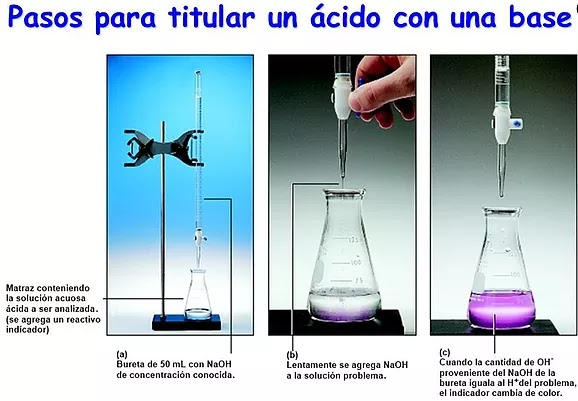
\includegraphics[width=.8\textwidth]{./Figures/titulacionManual.jpg}
	\caption{Titulación ácido-base manual mediante indicador de color\protect\footnotemark.}
	\label{fig:titManualColor}
\end{figure}



El cambio en el potencial de un electrodo de pH es la técnica que se utilizó para este trabajo y se detalla en la  figura \ref{fig:titManualPot}. En la imagen se observa un proceso manual asistido por una computadora que registra los datos de la cantidad de gotas que añade el usuario y el valor de pH leído por el electrodo.

\footnotetext{Imagen tomada de \url{https://2.bp.blogspot.com/-a9RepHphLgc/WgOVnU_U_QI/AAAAAAAAAGM/ulzSDSrbOKYNvtwqNhe_D5TE6bzxiT9aACLcBGAs/s1600/acido-base.webp}}

\begin{figure}[htbp]
	\centering
	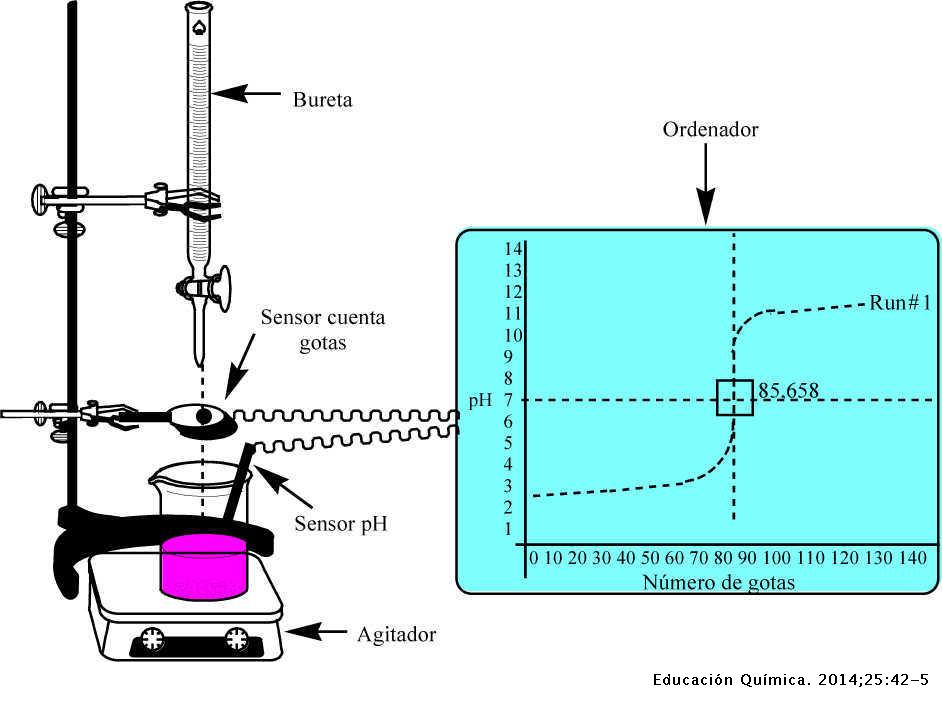
\includegraphics[width=.7\textwidth]{./Figures/titulacionPotManual.jpeg}
	\caption{Titulación ácido-base manual mediante indicador de color\protect\footnotemark.}
	\label{fig:titManualPot}
\end{figure}

\footnotetext{Imagen tomada de \url{https://www.elsevier.es/es-revista-educacion-quimica-78-articulo-titulaciones-acido-base-con-el-empleo-S0187893X14705221}}

\subsection{Curvas de titulación}

Una curva de titulación es una gráfica de alguna variable asociada a la concentración en función del volumen de titulante agregado. Generalmente se dan dos tipos de curvas: la sigmoidea y la de segmento lineal \citep{BOOK:1}.
Para el trabajo desarrollado se tuvo en cuenta la curva del tipo sigmoidea, como se muestra en la figura \ref{fig:sigmoidea}. En la misma se observa que el punto de equivalencia coincide con el punto de inflexión de la curva, característica que permite determinar de manera aproximada el punto final. 

\begin{figure}[htbp]
	\centering
	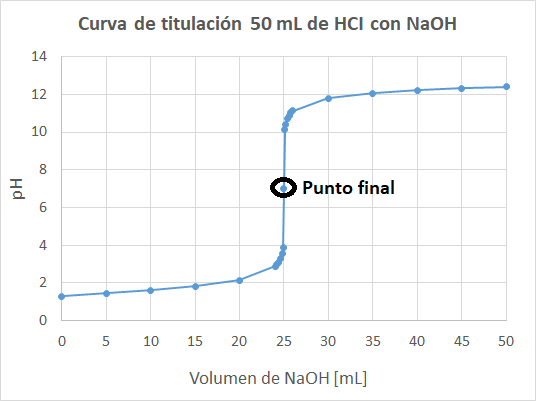
\includegraphics[width=.5\textwidth]{./Figures/curvaTitulacion1.png}
	\caption{Curva de titulación del tipo sigmoidea\protect\footnotemark.}
	\label{fig:sigmoidea}
\end{figure}

\footnotetext{Imagen tomada de \url{https://www.lifeder.com/punto-de-equivalencia/}}

\subsection{Potenciometría}

La potenciometría se basa en la medición del potencial de celdas electroquímicas  con corriente despreciable. Para llevar a cabo se utilizan dos electrodos: un electrodo de referencia con potencial conocido e independiente de la solución analizada, y un electrodo indicador cuya tensión varía en función de la actividad del analito,  separados por un puente salino que previene que los componentes de la disolución de analito se mezclen con los componentes del electrodo de referencia, tal y como se muestra en la figura \ref{fig:potenciometria} \citep{BOOK:1}.

\begin{figure}[htbp]
	\centering
	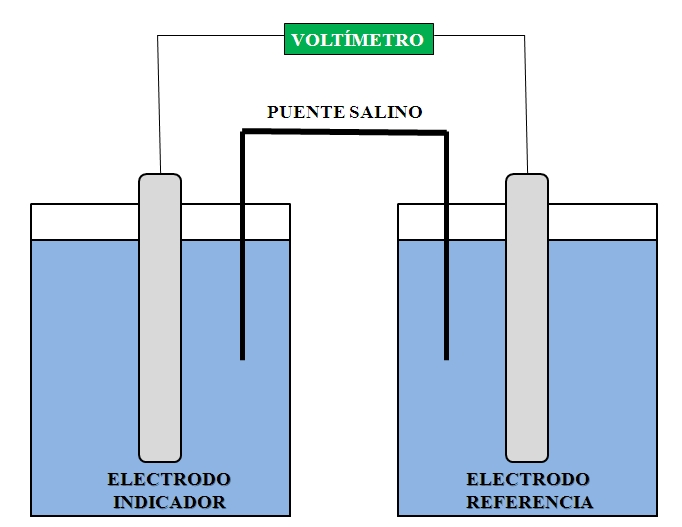
\includegraphics[width=.5\textwidth]{./Figures/Potenciometria-img.jpg}
	\caption{Curva de titulación del tipo sigmoidea\protect\footnotemark.}
	\label{fig:potenciometria}
\end{figure}

\footnotetext{Imagen tomada de \url{https://www.lifeder.com/potenciometria/}}
%----------------------------------------------------------------------------------------
\section{Descripción de tituladores automáticos}
\label{tituladoresAutomaticos}

Un titulador automático es un dispositivo que agrega titulante en la solución a analizar y registra alguna variable física por cada unidad de volumen o masa de titulante agregada. En base a esos datos, se puede elaborar la curva de titulación y calcular el volumen o masa en el punto final.
Existen diferentes tipos de tituladores que se usan para diferentes análisis, como por ejemplo el titulador potenciométrico, el de conductividad, Karl Fischer, entre otros.

Un titulador potenciométrico automático hace uso de un electrodo para medir el potencial de la celda a la vez que inyecta el titulante mediante el uso de algún sistema de dosificación, y registra cada valor potencial en mV o en pH en función de la cantidad de volumen añadido. Además, estos dispositivos suelen incluir un agitador que permite acelerar el proceso de mezcla entre el titulante añadido y la solución, para que el cambio en el potencial se visualice de manera más rápida.
En la figura \ref{fig:titThermo} se observa un ejemplo de un titulador comercial para titulaciones del tipo ácido-base.

\begin{figure}[htbp]
	\centering
	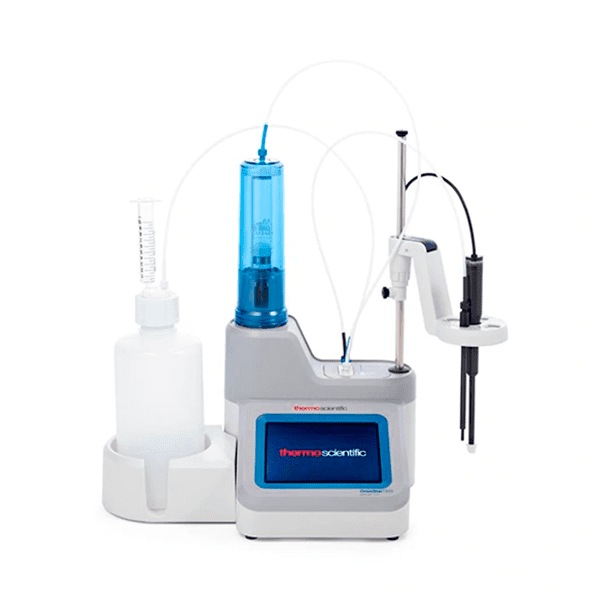
\includegraphics[width=.6\textwidth]{./Figures/titThermo.png}
	\caption{Ejemplo de titulador automático. Marca THERMO SCIENTIFIC\protect\footnotemark.}
	\label{fig:titThermo}
\end{figure}

\footnotetext{Imagen tomada de \url{https://www.equiposylaboratorio.com/portal/productos/titulador-automAtico-thermo-scientific-start9100-orion-star-t910}}



%----------------------------------------------------------------------------------------
\section{Estado del arte}

Existen gran variedad de tituladores potenciométricos automáticos en el mercado con diferentes características. La tabla \ref{tab:titComerciales} ilustra una comparativa entre algunos modelos de tituladores que disponen diferentes laboratorios de la región. \textbf{(acá podría explicar el contenido de la tabla)}

\begin{table}[h]
	\centering
	\caption[caption corto]{Comparativa de tituladores comerciales}
	\begin{tabular}{l c c}    
		\toprule
		\textbf{Marca} 	 & \textbf{Modelo} 		& \textbf{Características}  \\
		\midrule
		Kem					 & AT510 			& a \\		
		Mettler Toledo		 & Compact			& b \\
		Hanna				 & HI901C1-01		& c \\
		\bottomrule
		\hline
	\end{tabular}
	\label{tab:titComerciales}
\end{table}

%----------------------------------------------------------------------------------------
\section{Motivación}
El desarrollo de un titulador automático surgió de la iniciativa del grupo de I+D GISAI perteneciente a la UTN FRSFco con el fin de encarar un proyecto multidisciplinar en el que se involucren las cuatro carreras de ingeniería de la facultad. Luego de confirmar los integrantes del proyecto, se decidió en conjunto construir un titulador de bajo costo para el laboratorio de servicios de química, ya que los tituladores comerciales son económicamente inaccesibles para universidades y laboratorios en los que existe una frecuencia baja de muestras a analizar.
Una vez planteado el proyecto, se dividieron los objetivos particulares de cada área disciplinar, los cuales se detallan a continuación:
\begin{itemize}
\item Ingeniería Química: encargada de establecer los requerimientos y de validar el prototipo.
\item Ingeniería Electrónica: encargada de diseñar e implementar el sistema embebido que controle el proceso de titulación.
\item Ingeniería Electromecánica: encargada de diseñar y desarrollar la bomba y otros componentes mecánicos, como ca carcasa.
\item Ingeniería en Sistemas de Información: encargada de elaborar el software que procesará los datos entregados por el titulador y otros datos asociados a la muestra analizada y al cliente que lo solicita.
\end{itemize}
En esta memoria se describen las tareas realizadas dentro del área de Ingeniería Electrónica, cuyos objetivos y alcances se encuentran detallados en la sección \ref{objYalc}.

%----------------------------------------------------------------------------------------
\section{Objetivos y alcance}
\label{objYalc}

El trabajo realizado consistió en desarrollar el prototipo de un sistema embebido que permita automatizar y controlar el método de titulación potenciométrica.

El trabajo incluye:
\begin{itemize}
\item Una interfaz de usuario que permite realizar las configuraciones correspondientes, calibrar el dispositivo, y dar inicio y fin al proceso de titulación.
\item La visualización de la curva de pH respecto al tiempo.
\item El control de la bomba que inyecta el titulante en la solución a analizar.
\item El cálculo y visualización del volumen del titulante en el punto final.
\item El almacenamiento de los datos del ensayo en una memoria SD.
\item La visualización de los datos del ensayo en una página web, a través de una conexión Wi-Fi local.
\end{itemize}

El trabajo no incluye:
\begin{itemize}
\item El manejo del dispositivo de manera remota.
\item El diseño de la carcasa u otras partes mecánicas. 
\end{itemize}

En el diagrama de la figura \ref{fig:diagramaBloqueSimple} se muestra como interactúa el sistema desarrollado con las partes intervinientes. El sistema embebido es el encargado de controlar el volumen de titulante que la bomba agrega a la solución, y de leer el valor de pH obtenido por el electrodo. Una vez obtenidos todos los valores del proceso, los almacena en una tabla y calcula el volumen correspondiente al punto final. Ambos datos son enviados al software de la computadora.

\begin{figure}[htbp]
	\centering
	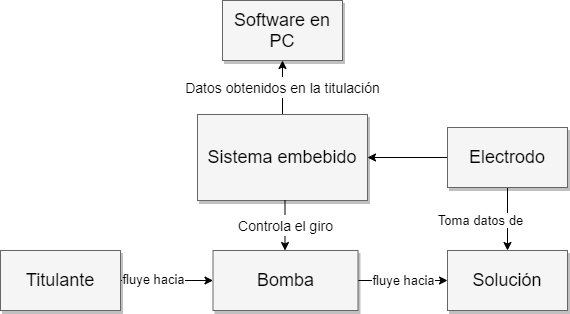
\includegraphics[width=.8\textwidth]{./Figures/DiagramaBloquesSimple.png}
	\caption{Diagrama en bloques simplificado.}
	\label{fig:diagramaBloqueSimple}
\end{figure}
\chapter{Introducción específica} % Main chapter title

\label{Chapter2}

%----------------------------------------------------------------------------------------
%	SECTION 1
%----------------------------------------------------------------------------------------
En este capítulo se  realiza un revisión detallada de los dispositivos y tecnologías utilizados y que fueron desarrollados por terceros para comprender las decisiones de diseño tomadas que se mencionan en el capítulo \ref{Chapter3}. 

%----------------------------------------------------------------------------------------
\section{Electrodos de pH}
\label{sec:electrodoPH}

Un electrodo muy usado hoy en día, es el electrodo combinado que está formado por dos electrodos dentro del mismo encapsulado. En la figura \ref{fig:electrodoCombinado} se observa un electrodo combinado que está formado por un electrodo de referencia, que consiste en un alambre clorurado de plata en una solución de KCl saturada, y un electrodo indicador, formado por el alambre clorurado de plata más una membrana de vidrio sensible al pH.

\begin{figure}[htbp]
	\centering
	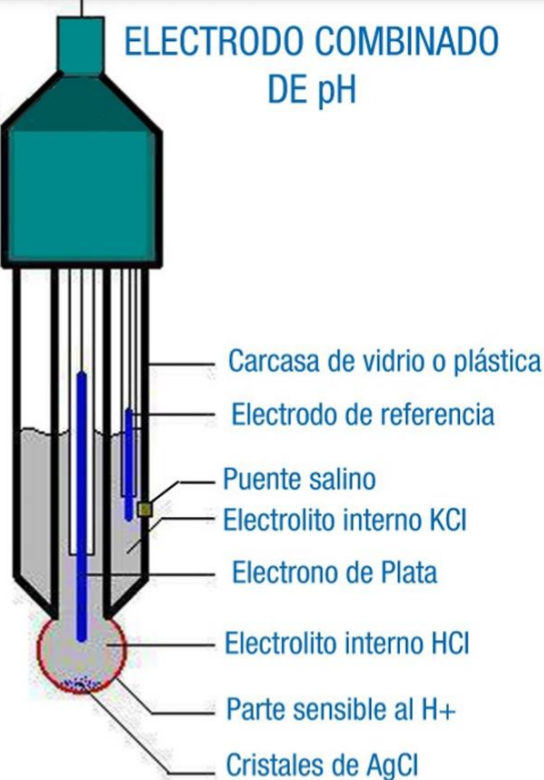
\includegraphics[width=.5\textwidth]{./Figures/electrodoCombinado.png}
	\caption{Electrodo combinado de pH de Ag/AgCl\protect\footnotemark.}
	\label{fig:electrodoCombinado}
\end{figure}

\footnotetext{Imagen tomada de \url{http://depa.fquim.unam.mx/amyd/archivero/ELECTRODOSDEMEDIDAYDEREFERENCIA_22645.pdf}}

El potencial de un electrodo está dado por la ecuación de Nernst, que se puede escribir de manera simplificada como muestra la ecuación \ref{eq:Nernst} .

\begin{equation}
	\label{eq:Nernst}
E = E_{0} + k pH
\end{equation}
\citep{ARTICLE:4}

donde E es el potencial corregido del electrodo, $E_{0}$ es el potencial en condiciones estándar (valores tabulados), k una variable que depende de la temperatura y pH es el valor de pH de la muestra.

En este trabajo se utilizó el electrodo comercial marca HANNA HI-1230B de la figura \ref{fig:hi-1230b}, definido por el área de Ingeniería Química, ya que permite realizar titulaciones potenciométricas ácido-base para detectar nitrógeno en suelo y alcalinidad en agua. Específicamente, este electrodo es de plata sumergido en una disolución de cloruro de potasio que se ha saturado con cloruro de plata, y presenta un potencial de 0 mV para un valor de pH de 7,01, y una pendiente de -0,0174pH/mV. En base a estos datos se puede crear la recta que relaciona la potencial del electrodo con el valor de pH y que está dada por la ecuación \ref{eq:phElectrodo}:

\begin{equation}
	\label{eq:phElectrodo}
pH = -0,0174 E + 7,01
\end{equation}

donde E es el potencial entregado por el electrodo y pH es el valor correspondiente de pH de la muestra a 25 °C. Para una muestra con ph 0 la salida del electrodo es de 402,8 mV y para una muestra de ph 14 el potencial es de -401,7 mV.

\begin{figure}[htbp]
	\centering
	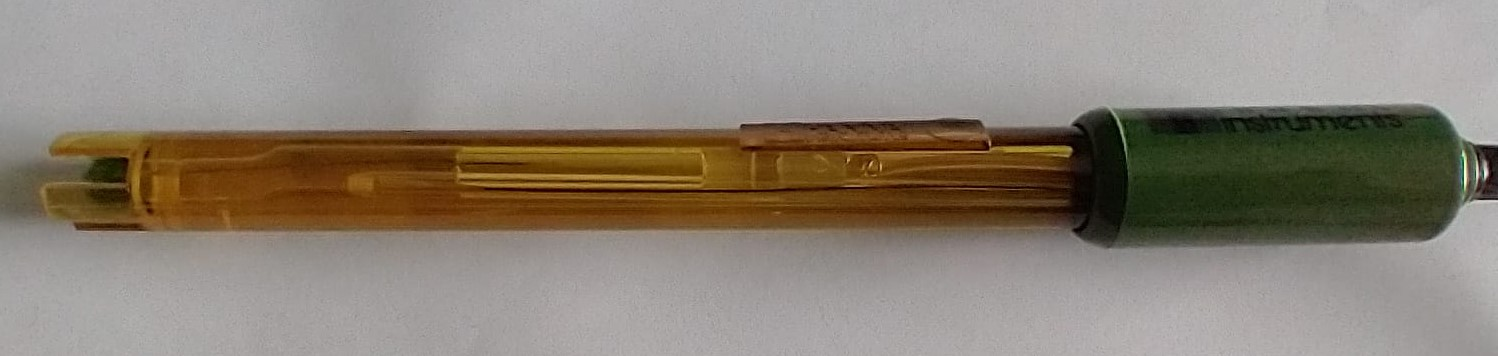
\includegraphics[width=.6\textwidth]{./Figures/hi-1230b.jpeg}
	\caption{Electrodo HI-1230B.}
	\label{fig:hi-1230b}
\end{figure}

%----------------------------------------------------------------------------------------
\section{Bombas peristálticas}
\label{sec:bomba}

Una bomba peristáltica es un tipo de bomba hidráulica que se emplea para transportar diferentes tipos de líquidos, y generalmente es usada cuando se emplean fluidos limpios o estériles ya que el mecanismo de la bomba no los contamina al desplazarlos \citep{ARTICLE:5}. Está formada por una manguera flexible situada dentro de la cubierta de la bomba, que puede ser circular o lineal, y un rotor compuesto por varios rodillos que comprimen la manguera, tal y como se muestra en la figura \ref{fig:bombaPeristEsq}. Cuando el rotor gira, se genera un vacío que hace que el líquido ingrese y fluya por la manguera.

\begin{figure}[htbp]
	\centering
	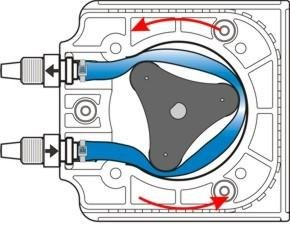
\includegraphics[width=.4\textwidth]{./Figures/bombaPeristEsq.png}
	\caption{Bomba peristáltica\protect\footnotemark.}
	\label{fig:bombaPeristEsq}
\end{figure}

\footnotetext{Imagen tomada de \url{https://www.researchgate.net/figure/Figura-3-Principio-de-funcionamiento-de-una-bomba-peristaltica-de-3-rodillos_fig2_275959587}}


Para este trabajo se utilizó la bomba desarrollada por el área de electromecánica, que hace uso de un motor paso a paso bipolar Nema 17 marca Usongshine, como se aprecia en la figura \ref{fig:bombaAtras}.

\begin{figure}[htbp]
	\centering
	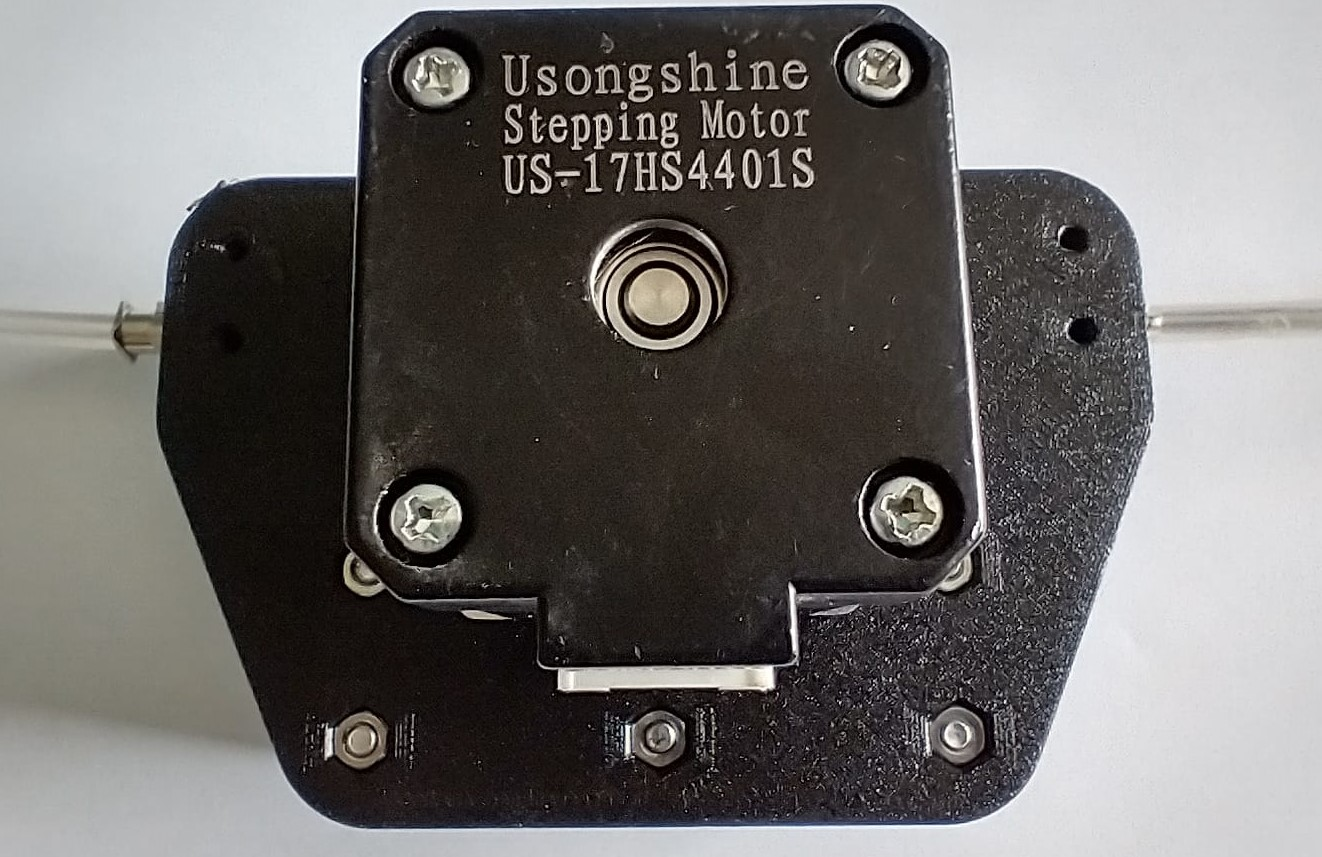
\includegraphics[width=.5\textwidth]{./Figures/bombaAtras.jpeg}
	\caption{Bomba peristáltica desarrollada por el área de Ingeniería Electromecánica. Vista del motor.}
	\label{fig:bombaAtras}
\end{figure}

La carcasa, el rotor y la cubierta exterior están impresas con ácido poliláctico (PLA) Grilon y contiene dos tipos de mangueras: una manguera PharMed BPT de 4 mm de diámetro exterior y 0,8 mm de diámetro interior que soporta las deformaciones cíclicas producidas por los rodillos del rotor, y dos mangueras genéricas de silicona para los tramos de entrada y salida. En las figura \ref{fig:bombaFrente} se observan los componentes mencionados.

\begin{figure}[htbp]
	\centering
	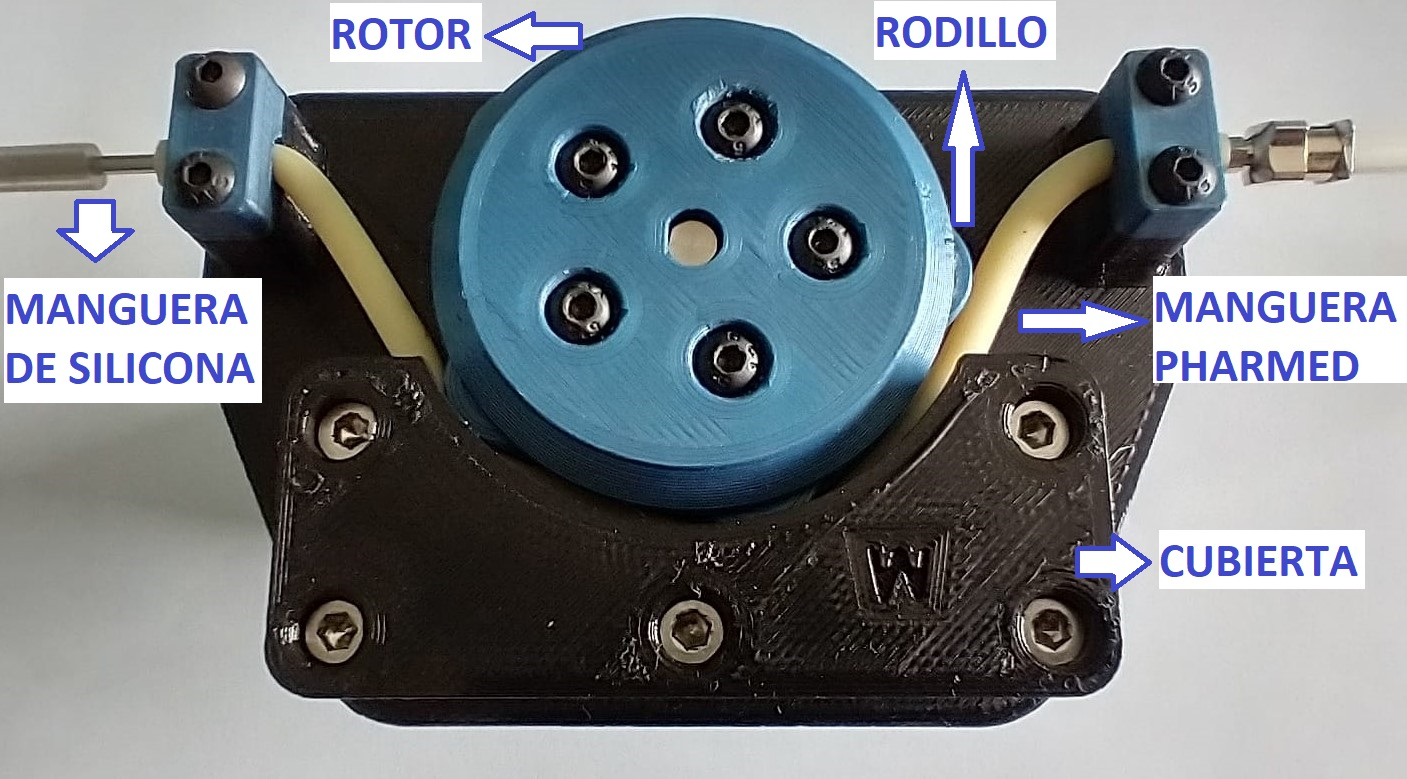
\includegraphics[width=.6\textwidth]{./Figures/bombaFrente.jpg}
	\caption{Bomba peristáltica desarrollada por el área de Ingeniería Electromecánica. Vista de los rodillos.}
	\label{fig:bombaFrente}
\end{figure}

%con un rango de voltaje apto de 5 a 36V, torque de 42 N.cm, máxima corriente 1,7A, de 1.8° por paso, lo que implica que para lograr una vuelta entera del eje (360°) el motor debe dar unos 200 pasos. 

%El diseño de las piezas mecánicas se basó en una bomba peristáltica de precisión. Para el modelado 3D se empleó el software SolidWorks®. La impresión de la carcasa, rotor y cubeta exterior se realizó con ácido poliláctico (PLA) Grilon.

%En relación con la selección de tubos flexibles o mangueras, se utilizaron dos tipos. Por un lado, una manguera PharMed BPT (de alta calidad, resistencia química, diseñada especialmente para aplicaciones de bombas peristálticas de 4 mm de diámetro exterior y 0,8 mm de diámetro interior), se empleó en la cubierta circular interior que posee la bomba y que soportará las deformaciones cíclicas producidas por los rodillos del rotor.

%Por otro lado, se utilizaron mangueras genéricas de silicona (de 4mm diámetro exterior y 0.8mm diámetro interior) para los tramos de entrada y salida de la bomba.

%----------------------------------------------------------------------------------------
\section{Otras tecnologías utilizadas}

Este trabajo se enfocó en el diseño de un prototipo de titulador, con el foco puesto en el software más que en el hardware. Es por eso que se buscaron alternativas del tipo "módulo" para los diferentes componentes, de tal forma que permita una rápida conexión del hardware y delegar la mayor parte del tiempo al desarrollo del firmware. En cada una de las siguientes secciones se describen los módulos utilizados.

\subsection{Microcontrolador ESP32}

Para el desarrollo del prototipo se utilizó la placa de desarrollo ESP32-DevKitC de la figura \ref{fig:ESP32.jpeg}. Esta placa contiene un módulo ESP32 con Wi-Fi y Bluetooth integrado y un sistema de doble núcleo, cada uno con un CPU Xtensa LX6 de 32 bit.

\begin{figure}[htbp]
	\centering
	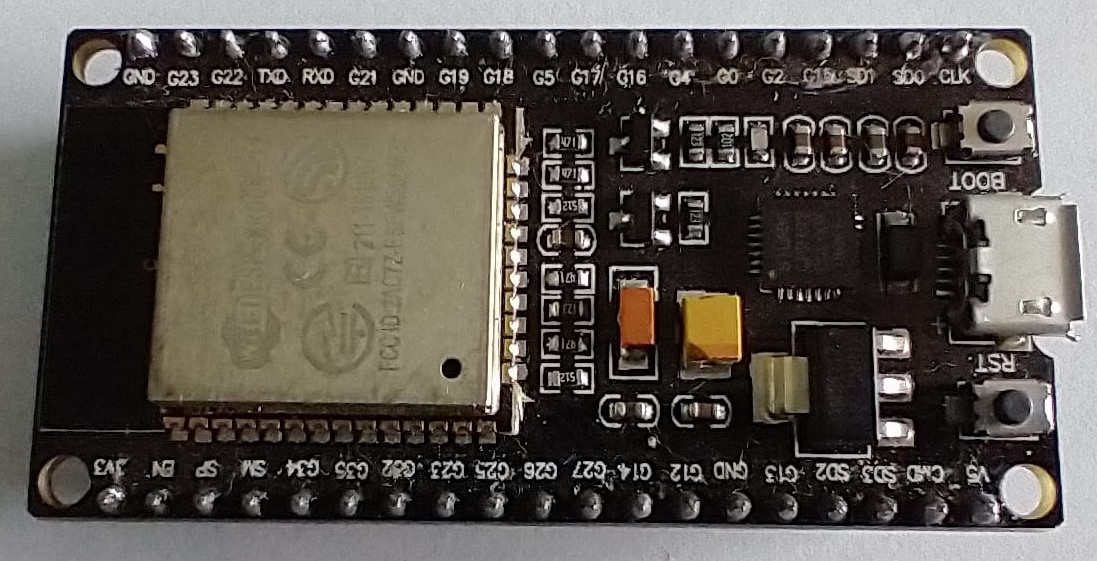
\includegraphics[width=.4\textwidth]{./Figures/ESP32.jpeg}
	\caption{Placa de desarrollo ESP32-DevKitC.}
	\label{fig:ESP32.jpeg}
\end{figure}

Las principales características de esta placa de desarrollo que se tuvieron en cuenta para el desarrollo del trabajo son las siguientes:
	\begin{itemize}
		\item Clock a 160 MHz.
		\item 4 MB de memoria flash.
		\item Wi-Fi: 802.11 b/g/n.
		\item 12-bit SAR ADC de hasta 18 canales.
		\item 3 × UART
		\item Controlador host SD
		\item PWM
	\end{itemize}

Para el desarrollo del software se utilizó el framework ESP-IDF de Espressif Systems, que ofrece una API para trabajar con una versión de FreeRTOS adaptada para aprovechar el doble núcleo del procesador, asi como también para el resto de los periféricos mencionados anteriormente.

\subsection{Pantalla táctil}

Los tituladores comerciales cuentan con una pantalla a través de la cuál se muestra una interfaz de usuario que permite acceder a las configuraciones y controlar las distintas funciones. En algunos casos la pantalla está acompañada por un teclado y en otros casos cuenta directamente con un panel táctil. Para este trabajo se decidió optar por la segunda opción ya que permite mayor flexibilidad a la hora de realizar cambios en la interfaz.

Entre las opciones disponibles en el mercado, se optó por módulo MCUFRIEND de la figura \ref{fig:LCDFrente} que contiene una pantalla LCD de 2,4" con un panel táctil y un lector de tarjetas SD.

\begin{figure}[htbp]
	\centering
	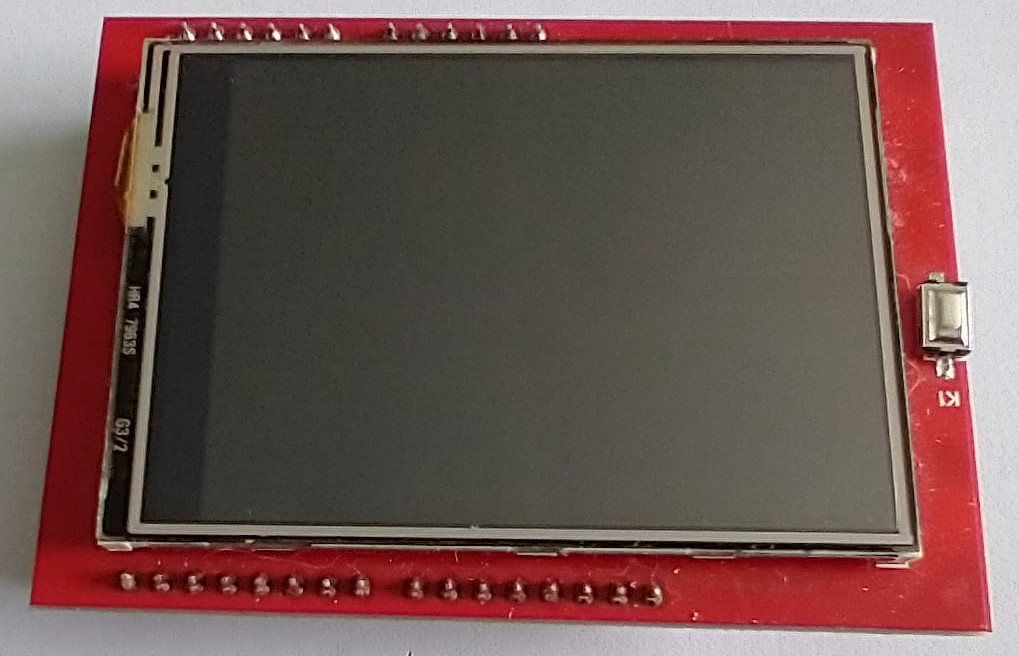
\includegraphics[width=.4\textwidth]{./Figures/LCDFrente.jpeg}
	\caption{LCD táctil MCUFRIEND.}
	\label{fig:LCDFrente}
\end{figure}

\subsection{\textit{Driver} para motor}

Previamente, en la sección \ref{sec:bomba}, se mencionó que la bomba utiliza un motor paso a paso. Para que el módulo ESP32 pueda controlarlo es necesario utilizar un \textit{driver} que otorgue los niveles de tensión y corriente necesarios para su correcto funcionamiento.

Para este trabajo se utilizó el módulo DRV8825 de la figura \ref{fig:DRV8825-Frente}, que permite el manejo de motores paso a paso de hasta 2,5 A y tiene la posibilidad de utilizar \textit{microsteping} 1/32.

\begin{figure}[htbp]
	\centering
	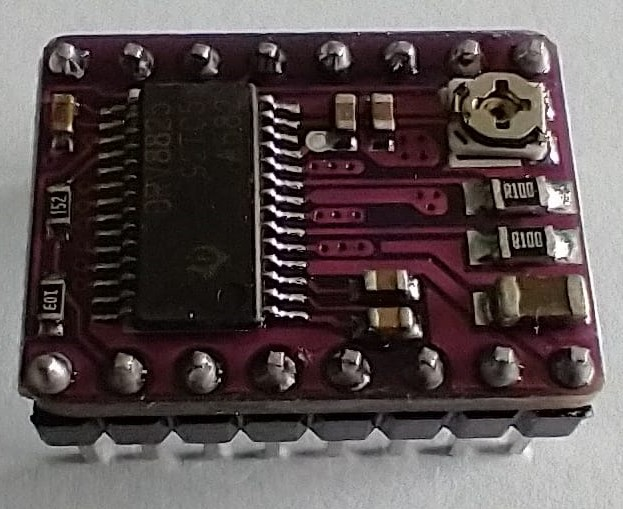
\includegraphics[width=.3\textwidth]{./Figures/DRV8825-Frente.jpeg}
	\caption{\textit{Driver} para motor paso a paso DRV8825.}
	\label{fig:DRV8825-Frente}
\end{figure}

La técnica de \textit{microsteping} permite multiplicar la cantidad de pasos que puede dar un motor para realizar una vuelta. De esta forma se puede aumentar la resolución de giro, es decir, disminuir el ángulo de paso del motor, lo que se traduce a una menor cantidad de volumen inyectada por cada paso.

\subsection{Módulo de adaptación para electrodo}

En la sección \ref{sec:electrodoPH} se mencionó que el electrodo entrega un potencial que va a depender del pH de la muestra y se ubica entre -401,7 y 402,8 mV. Para poder procesar estos valores con el ADC del ESP32, cuyo rango de entrada es de 0 a 3500 mV, es necesario adaptar esa señal para amplificar la tensión y adaptar impedancias. Para eso se utilizó el módulo pH-4502C de la figura \ref{fig:pH-4502C}.

\begin{figure}[htbp]
	\centering
	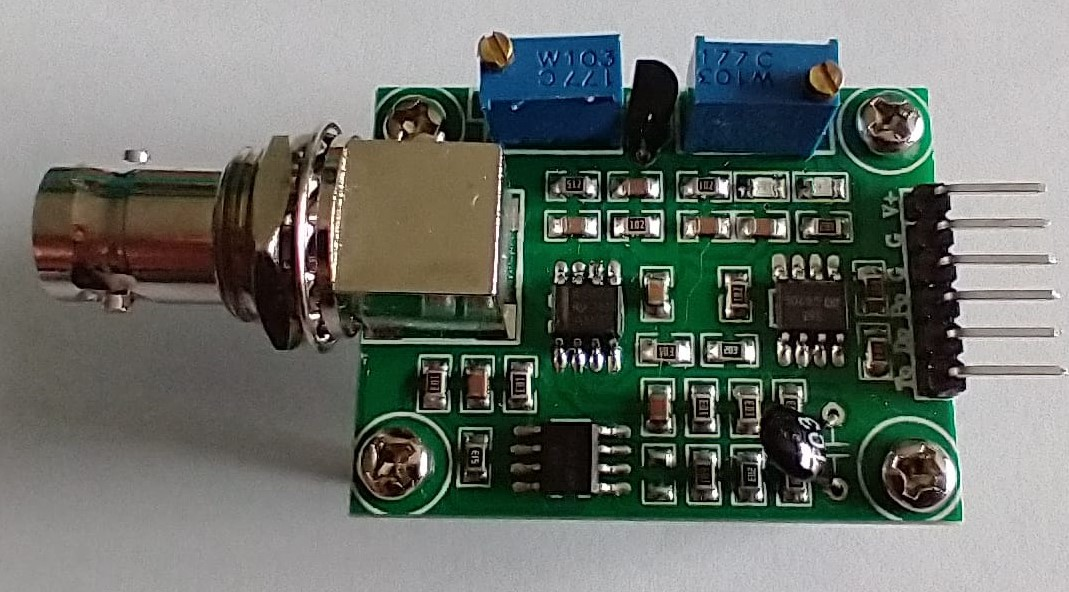
\includegraphics[width=.4\textwidth]{./Figures/pH-4502C.jpeg}
	\caption{Módulo pH-4502C.}
	\label{fig:pH-4502C}
\end{figure}

El módulo PH-4502C está formado por dos etapas. En la Fig. 4 se observa la etapa de amplificación de la señal, la cual utiliza un amplificador operacional con una configuración del tipo no inversor y con una ganancia de 2. En la Fig. 5 se muestra la etapa que permite regular la tensión de referencia. Está formado por un amplificador operacional en configuración de seguidor de tensión y un divisor resistivo con un potenciómetro que permite calibrar el nivel de tensión para evitar valores negativos en la salida del circuito.

%----------------------------------------------------------------------------------------
\section{Requerimientos}
\label{sec:requerimientos}

En esta sección se detallan los requerimientos del sistema que fueron planteados en el plan trabajo, con ligeros cambios que surgieron durante el desarrollo del trabajo.

\begin{itemize}
\item Interfaces Externas
	\begin{itemize}
	\item El hardware debe contar con una pantalla TFT táctil. [TPA-ERH-01-REQ001]
	\item El hardware debe contar con un lector de tarjetas SD. [TPA-ERH-01-REQ002]
	\item El hardware debe contar con un \textit{driver} para un motor paso a paso Nema 17. [TPA-ERH-01-REQ003]
	\item El hardware debe contar con una entrada para un electrodo de pH. [TPA-ERH-01-REQ004]
	\end{itemize}
	
\item Funciones
	\begin{itemize}
	\item El usuario debe poder elegir mediante la pantalla táctil el volumen de corte de la titulación. [TPA-ERS-01-REQ001]
	\item El usuario debe poder elegir mediante la pantalla táctil si utilizar o no el agitador. Cuando el proceso de titulación comienza, el agitador debe activarse si así lo indicó el usuario. [TPA-ERS-01-REQ002]
	\item El usuario debe poder realizar mediante la pantalla táctil el proceso de calibración con cada uno de los tres buffers. [TPA-ERS-01-REQ003]
	\item Los valores de potencial obtenidos en el proceso de la calibración se deben guardar en la memoria flash del ESP32. [TPA-ERS-01-REQ004]
	\item El valor de pH se debe calcular de manera proporcional a la recta de ajuste de los valores de potencial obtenidos en la calibración. [TPA-ERS-01-REQ005]
	\item El usuario debe poder dar inicio al proceso de titulación mediante la pantalla táctil. [TPA-ERS-01-REQ006]
	\item Durante la titulación, la pantalla debe mostrar el valor actual leído en mV y en pH y una gráfica de pH en función del tiempo. [TPA-ERS-01-REQ007]
	\item Cada valor de volumen añadido junto al valor de potencial asociado durante el proceso de titulación deben almacenarse en un archivo de texto en la tarjeta sd. No es necesario que esto se haga en tiempo real. [TPA-ERS-01-REQ008]
	\item Cada valor de volumen añadido junto al valor de potencial asociado durante el proceso de titulación deben mostrarse en una página web almacenada en la memoria flash, una vez finalizada la titulación. [TPA-ERS-01-REQ009]
	\item El usuario debe poder acceder a la página web mediante una conexión Wi-Fi. No es necesario que esto se haga en tiempo real. [TPA-ERS-01-REQ010]
	\item El sistema debe ser capaz de leer y mostrar el potencial entregado por un electrodo de pH, con una resolución de 1 mV para la lectura del potencial y de 0,01 pH para su conversión a pH. [TPA-ERS-01-REQ011]
	\item El sistema deberá inyectar una cantidad de 0,1 mL y luego esperar 5 segundos para realizar la medición de pH. La cantidad inyectada puede ser de 1 mL si el cambio de ph entre las últimas dos mediciones es menor a 0,2. [TPA-ERS-01-REQ012]
	 \item El sistema debe dejar de agregar titulante cuando se alcanza la cantidad de volumen indicada por el usuario como volumen de corte. [TPA-ERS-01-REQ013]

\end{itemize}

\item Requisitos de Rendimiento
	\begin{itemize}
	\item El sistema debe ser capaz de realizar titulaciones que involucren una cantidad máxima de 100 ml. [TPA-ERS-01-REQ014]
	\end{itemize}
	
\item Restricciones de Diseño
	\begin{itemize}
	\item Se utiliza el módulo ESP32 como computadora principal. [TPA-ERS-01-REQ015]
	\item Se utiliza la pantalla táctil MCUFRIEND 2,4'' como interfaz de usuario. [TPA-ERS-01-REQ016]
	\end{itemize}
\end{itemize}	
%----------------------------------------------------------------------------------------
% TODO LO DE ACÁ ABAJO ES EL MODELO

%\section{Estilo y convenciones}
%\label{sec:ejemplo}
%
%\subsection{Uso de mayúscula inicial para los título de secciones}
%
%Si en el texto se hace alusión a diferentes partes del trabajo referirse a ellas como capítulo, sección o subsección según corresponda. Por ejemplo: ``En el capítulo \ref{Chapter1} se explica tal cosa'', o ``En la sección \ref{sec:ejemplo} se presenta lo que sea'', o ``En la subsección \ref{subsec:ejemplo} se discute otra cosa''.
%
%Cuando se quiere poner una lista tabulada, se hace así:
%
%\begin{itemize}
%	\item Este es el primer elemento de la lista.
%	\item Este es el segundo elemento de la lista.
%\end{itemize}
%
%Notar el uso de las mayúsculas y el punto al final de cada elemento.
%
%Si se desea poner una lista numerada el formato es este:
%
%\begin{enumerate}
%	\item Este es el primer elemento de la lista.
%	\item Este es el segundo elemento de la lista.
%\end{enumerate}
%
%Notar el uso de las mayúsculas y el punto al final de cada elemento.
%
%\subsection{Este es el título de una subsección}
%\label{subsec:ejemplo}
%
%Se recomienda no utilizar \textbf{texto en negritas} en ningún párrafo, ni tampoco texto \underline{subrayado}. En cambio sí se debe utilizar \textit{texto en itálicas} para palabras en un idioma extranjero, al menos la primera vez que aparecen en el texto. En el caso de palabras que estamos inventando se deben utilizar ``comillas'', así como también para citas textuales. Por ejemplo, un \textit{digital filter} es una especie de ``selector'' que permite separar ciertos componentes armónicos en particular.
%
%La escritura debe ser impersonal. Por ejemplo, no utilizar ``el diseño del firmware lo hice de acuerdo con tal principio'', sino ``el firmware fue diseñado utilizando tal principio''. 
%
%El trabajo es algo que al momento de escribir la memoria se supone que ya está concluido, entonces todo lo que se refiera a hacer el trabajo se narra en tiempo pasado, porque es algo que ya ocurrió. Por ejemplo, "se diseñó el firmware empleando la técnica de test driven development".
%
%En cambio, la memoria es algo que está vivo cada vez que el lector la lee. Por eso transcurre siempre en tiempo presente, como por ejemplo:
%
%``En el presente capítulo se da una visión global sobre las distintas pruebas realizadas y los resultados obtenidos. Se explica el modo en que fueron llevados a cabo los test unitarios y las pruebas del sistema''.
%
%Se recomienda no utilizar una sección de glosario sino colocar la descripción de las abreviaturas como parte del mismo cuerpo del texto. Por ejemplo, RTOS (\textit{Real Time Operating System}, Sistema Operativo de Tiempo Real) o en caso de considerarlo apropiado mediante notas a pie de página.
%
%Si se desea indicar alguna página web utilizar el siguiente formato de referencias bibliográficas, dónde las referencias se detallan en la sección de bibliografía de la memoria, utilizado el formato establecido por IEEE en \citep{IEEE:citation}. Por ejemplo, ``el presente trabajo se basa en la plataforma EDU-CIAA-NXP \citep{CIAA}, la cual...''.
%
%\subsection{Figuras} 
%
%Al insertar figuras en la memoria se deben considerar determinadas pautas. Para empezar, usar siempre tipografía claramente legible. Luego, tener claro que \textbf{es incorrecto} escribir por ejemplo esto: ``El diseño elegido es un cuadrado, como se ve en la siguiente figura:''
%
%\begin{figure}[h]
%\centering
%\includegraphics[scale=.45]{./Figures/cuadradoAzul.png}
%\end{figure}
%
%La forma correcta de utilizar una figura es con referencias cruzadas, por ejemplo: ``Se eligió utilizar un cuadrado azul para el logo, como puede observarse en la figura \ref{fig:cuadradoAzul}''.
%
%\begin{figure}[ht]
%	\centering
%	\includegraphics[scale=.45]{./Figures/cuadradoAzul.png}
%	\caption{Ilustración del cuadrado azul que se eligió para el diseño del logo.}
%	\label{fig:cuadradoAzul}
%\end{figure}
%
%El texto de las figuras debe estar siempre en español, excepto que se decida reproducir una figura original tomada de alguna referencia. En ese caso la referencia de la cual se tomó la figura debe ser indicada en el epígrafe de la figura e incluida como una nota al pie, como se ilustra en la figura \ref{fig:palabraIngles}.
%
%\begin{figure}[htpb]
%	\centering
%	\includegraphics[scale=.3]{./Figures/word.jpeg}
%	\caption{Imagen tomada de la página oficial del procesador\protect\footnotemark.}
%	\label{fig:palabraIngles}
%\end{figure}
%
%\footnotetext{Imagen tomada de \url{https://goo.gl/images/i7C70w}}
%
%La figura y el epígrafe deben conformar una unidad cuyo significado principal pueda ser comprendido por el lector sin necesidad de leer el cuerpo central de la memoria. Para eso es necesario que el epígrafe sea todo lo detallado que corresponda y si en la figura se utilizan abreviaturas entonces aclarar su significado en el epígrafe o en la misma figura.
%
%
%
%\begin{figure}[ht]
%	\centering
%	\includegraphics[scale=.37]{./Figures/questionMark.png}
%	\caption{¿Por qué de pronto aparece esta figura?}
%	\label{fig:questionMark}
%\end{figure}
%
%Nunca colocar una figura en el documento antes de hacer la primera referencia a ella, como se ilustra con la figura \ref{fig:questionMark}, porque sino el lector no comprenderá por qué de pronto aparece la figura en el documento, lo que distraerá su atención.
%
%Otra posibilidad es utilizar el entorno \textit{subfigure} para incluir más de una figura, como se puede ver en la figura \ref{fig:three graphs}. Notar que se pueden referenciar también las figuras internas individualmente de esta manera: \ref{fig:1de3}, \ref{fig:2de3} y \ref{fig:3de3}.
% 
%\begin{figure}[!htpb]
%     \centering
%     \begin{subfigure}[b]{0.3\textwidth}
%         \centering
%         \includegraphics[width=.65\textwidth]{./Figures/questionMark}
%         \caption{Un caption.}
%         \label{fig:1de3}
%     \end{subfigure}
%     \hfill
%     \begin{subfigure}[b]{0.3\textwidth}
%         \centering
%         \includegraphics[width=.65\textwidth]{./Figures/questionMark}
%         \caption{Otro.}
%         \label{fig:2de3}
%     \end{subfigure}
%     \hfill
%     \begin{subfigure}[b]{0.3\textwidth}
%         \centering
%         \includegraphics[width=.65\textwidth]{./Figures/questionMark}
%         \caption{Y otro más.}
%         \label{fig:3de3}
%     \end{subfigure}
%        \caption{Tres gráficos simples}
%        \label{fig:three graphs}
%\end{figure}
%
%El código para generar las imágenes se encuentra disponible para su reutilización en el archivo \file{Chapter2.tex}.
%
%\subsection{Tablas}
%
%Para las tablas utilizar el mismo formato que para las figuras, sólo que el epígrafe se debe colocar arriba de la tabla, como se ilustra en la tabla \ref{tab:peces}. Observar que sólo algunas filas van con líneas visibles y notar el uso de las negritas para los encabezados.  La referencia se logra utilizando el comando \verb|\ref{<label>}| donde label debe estar definida dentro del entorno de la tabla.
%
%\begin{verbatim}
%\begin{table}[h]
%	\centering
%	\caption[caption corto]{caption largo más descriptivo}
%	\begin{tabular}{l c c}    
%		\toprule
%		\textbf{Especie}     & \textbf{Tamaño} & \textbf{Valor}\\
%		\midrule
%		Amphiprion Ocellaris & 10 cm           & \$ 6.000 \\		
%		Hepatus Blue Tang    & 15 cm           & \$ 7.000 \\
%		Zebrasoma Xanthurus  & 12 cm           & \$ 6.800 \\
%		\bottomrule
%		\hline
%	\end{tabular}
%	\label{tab:peces}
%\end{table}
%\end{verbatim}
%
%
%\begin{table}[h]
%	\centering
%	\caption[caption corto]{caption largo más descriptivo}
%	\begin{tabular}{l c c}    
%		\toprule
%		\textbf{Especie} 	 & \textbf{Tamaño} 		& \textbf{Valor}  \\
%		\midrule
%		Amphiprion Ocellaris & 10 cm 				& \$ 6.000 \\		
%		Hepatus Blue Tang	 & 15 cm				& \$ 7.000 \\
%		Zebrasoma Xanthurus	 & 12 cm				& \$ 6.800 \\
%		\bottomrule
%		\hline
%	\end{tabular}
%	\label{tab:peces}
%\end{table}
%
%En cada capítulo se debe reiniciar el número de conteo de las figuras y las tablas, por ejemplo, figura 2.1 o tabla 2.1, pero no se debe reiniciar el conteo en cada sección. Por suerte la plantilla se encarga de esto por nosotros.
%
%\subsection{Ecuaciones}
%\label{sec:Ecuaciones}
%
%Al insertar ecuaciones en la memoria dentro de un entorno \textit{equation}, éstas se numeran en forma automática  y se pueden referir al igual que como se hace con las figuras y tablas, por ejemplo ver la ecuación \ref{eq:metric}.
%
%\begin{equation}
%	\label{eq:metric}
%	ds^2 = c^2 dt^2 \left( \frac{d\sigma^2}{1-k\sigma^2} + \sigma^2\left[ d\theta^2 + \sin^2\theta d\phi^2 \right] \right)
%\end{equation}
%                                                        
%Es importante tener presente que si bien las ecuaciones pueden ser referidas por su número, también es correcto utilizar los dos puntos, como por ejemplo ``la expresión matemática que describe este comportamiento es la siguiente:''
%
%\begin{equation}
%	\label{eq:schrodinger}
%	\frac{\hbar^2}{2m}\nabla^2\Psi + V(\mathbf{r})\Psi = -i\hbar \frac{\partial\Psi}{\partial t}
%\end{equation}
%
%Para generar la ecuación \ref{eq:metric} se utilizó el siguiente código:
%
%\begin{verbatim}
%\begin{equation}
%	\label{eq:metric}
%	ds^2 = c^2 dt^2 \left( \frac{d\sigma^2}{1-k\sigma^2} + 
%	\sigma^2\left[ d\theta^2 + 
%	\sin^2\theta d\phi^2 \right] \right)
%\end{equation}
%\end{verbatim}
%
%Y para la ecuación \ref{eq:schrodinger}:
%
%\begin{verbatim}
%\begin{equation}
%	\label{eq:schrodinger}
%	\frac{\hbar^2}{2m}\nabla^2\Psi + V(\mathbf{r})\Psi = 
%	-i\hbar \frac{\partial\Psi}{\partial t}
%\end{equation}
%
%\end{verbatim}
 
\chapter{Diseño e implementación} % Main chapter title

\label{Chapter3} % Change X to a consecutive number; for referencing this chapter elsewhere, use \ref{ChapterX}

\definecolor{mygreen}{rgb}{0,0.6,0}
\definecolor{mygray}{rgb}{0.5,0.5,0.5}
\definecolor{mymauve}{rgb}{0.58,0,0.82}

%%%%%%%%%%%%%%%%%%%%%%%%%%%%%%%%%%%%%%%%%%%%%%%%%%%%%%%%%%%%%%%%%%%%%%%%%%%%%
% parámetros para configurar el formato del código en los entornos lstlisting
%%%%%%%%%%%%%%%%%%%%%%%%%%%%%%%%%%%%%%%%%%%%%%%%%%%%%%%%%%%%%%%%%%%%%%%%%%%%%
\lstset{ %
  backgroundcolor=\color{white},   % choose the background color; you must add \usepackage{color} or \usepackage{xcolor}
  basicstyle=\footnotesize,        % the size of the fonts that are used for the code
  breakatwhitespace=false,         % sets if automatic breaks should only happen at whitespace
  breaklines=true,                 % sets automatic line breaking
  captionpos=b,                    % sets the caption-position to bottom
  commentstyle=\color{mygreen},    % comment style
  deletekeywords={...},            % if you want to delete keywords from the given language
  %escapeinside={\%*}{*)},          % if you want to add LaTeX within your code
  %extendedchars=true,              % lets you use non-ASCII characters; for 8-bits encodings only, does not work with UTF-8
  %frame=single,	                % adds a frame around the code
  keepspaces=true,                 % keeps spaces in text, useful for keeping indentation of code (possibly needs columns=flexible)
  keywordstyle=\color{blue},       % keyword style
  language=[ANSI]C,                % the language of the code
  %otherkeywords={*,...},           % if you want to add more keywords to the set
  numbers=left,                    % where to put the line-numbers; possible values are (none, left, right)
  numbersep=5pt,                   % how far the line-numbers are from the code
  numberstyle=\tiny\color{mygray}, % the style that is used for the line-numbers
  rulecolor=\color{black},         % if not set, the frame-color may be changed on line-breaks within not-black text (e.g. comments (green here))
  showspaces=false,                % show spaces everywhere adding particular underscores; it overrides 'showstringspaces'
  showstringspaces=false,          % underline spaces within strings only
  showtabs=false,                  % show tabs within strings adding particular underscores
  stepnumber=1,                    % the step between two line-numbers. If it's 1, each line will be numbered
  stringstyle=\color{mymauve},     % string literal style
  tabsize=2,	                   % sets default tabsize to 2 spaces
  title=\lstname,                  % show the filename of files included with \lstinputlisting; also try caption instead of title
  morecomment=[s]{/*}{*/}
}
%----------------------------------------------------------------------------------------

En este capítulo se detallan los componentes de \textit{firmware} y hardware diseñados e implementados, su interrelación, y los criterios seguidos.

%----------------------------------------------------------------------------------------
%	SECTION 1
%----------------------------------------------------------------------------------------
\section{Arquitectura del sistema}

Para abordar el trabajo realizado, en esta sección se expone la arquitectura general del sistema embebido implementado, esquematizada en el diagrama de la figura \ref{fig:diagramaCompleto}. Luego, en las siguientes secciones, se detallan cada uno de los componentes de manera individual.

\begin{figure}[htbp]
	\centering
	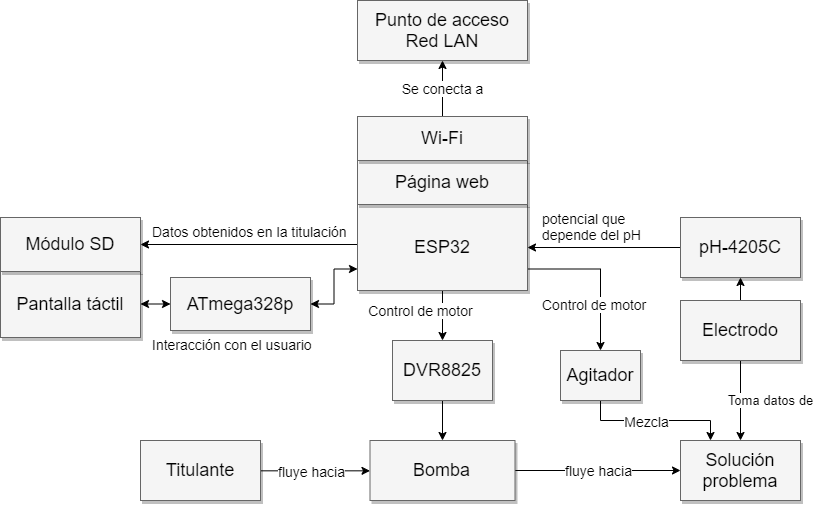
\includegraphics[width=1.0\textwidth]{./Figures/DiagramaBloquesCompleto.png}
	\caption{Diagrama en bloques del trabajo realizado.}
	\label{fig:diagramaCompleto}
\end{figure}

El componente principal del sistema es el ESP32, que tiene como función coordinar cada una de las partes intervinientes. A través de una comunicación del tipo UART con el ATmega328p, recibe las órdenes ingresadas a través de la pantalla táctil para realizar las configuraciones o funciones que solicite el usuario.

Por otro lado, el ESP32 realiza el control del motor de la bomba a través del \textit{driver} DVR8825. La bomba se utiliza en dos procesos: limpieza y titulación. La limpieza se utiliza para purgar la bomba previo al proceso de titulación y para eliminar los restos de titulante que quedan en las mangueras al finalizar el proceso.

Otra de las funciones del ESP32 es realizar la medición del pH de la muestra. Para eso utiliza el conversor ADC para leer el valor de potencial que entrega el módulo pH-4205C. Esta medición se utiliza en la calibración y en la titulación.

Por último, el ESP32 se encarga de registrar las mediciones de pH y cantidad de volumen que dosifica la bomba. Estos valores se alamacenan en un archivo de texto en una memoria micro SD y también puede ser visualizados a través de una pagina web.

Para realizar las actividades mencionadas previamente, el ESP32 ejecuta tres tareas: la tarea encargada de la comunicación UART con el ATmega328p, que se ejecuta en el núcleo 0, y las tareas de medición del electrodo y de control de la bomba, que se ejecutan en el núcleo 1. Además, existe un controlador de eventos, que se ejecuta sobre el núcleo 0 cuando alguien accede a la página web.
En las siguientes secciones estas tareas son desarrolladas con mayor profundidad.

%----------------------------------------------------------------------------------------
\section{Medición del electrodo}

La medición del electrodo se ejecuta en el contexto de una tarea de FreeRTOS. El objetivo de esta tarea es obtener el valor del conversor ADC, que proviene del módulo pH-4502C, y es ejecutada durante los procesos de calibración y de titulación. En el código \ref{cod:tareaElectrodo} se muestra el pseudocódigo de la tarea de medición del electrodo. En la línea 4 se realiza la configuración del ADC utilizado, el cual se habilita con una resolución de 12 bits en el pin correspondiente al canal 6 del ADC número 1.

La lectura del valor del ADC se acumula en la variable sumaAdc durante las N iteraciones del bucle \textit{for} de la línea 9. Estas iteraciones se realizan cada un intervalo de 10 ms y, al finalizar el bucle \textit{for}, el valor total se divide por la cantidad de muestras realizadas, como se muestra en la línea 15. Esto permite promediar el valor leído y así reducir el ruido presente en la conversión, tal y como sugiere la página oficial del ESP32 \citep{WEBSITE:2}. Cabe destacar que el acceso a la variable valorAdc está protegido por una sección crítica, entre líneas 14 y 16, ya que el resto de las tareas también pueden acceder a la variable cuando precisan calcular el valor de pH.

\begin{lstlisting}[label=cod:tareaElectrodo,caption=Pseudocódigo de la tarea de medición de pH.]
void tareaElectrodo (void *arg)
{
    //Configuracion de resolucion y pin del ADC
    configuracionADC(12 bits, pin);
    uint32_t sumaAdc = 0;

    while(true)
    {
    		for (int i=0; i< N_MUESTRAS; i++)
    		{
        		sumaAdc = sumaAdc + lecturaADC(pin);  
        		vTaskDelay(10 mS);
    		} 
    		inicioSeccionCritica(); 
    		valorAdc = sumaAdc / N_MUESTRAS;
    		finSeccionCritica();
    		sumaAdc = 0;
    }
}
\end{lstlisting}

%----------------------------------------------------------------------------------------
\section{Proceso de calibración}

En todo equipo de medición es importante asegurar que los valores sean confiables a lo largo del tiempo. Debido a que las propiedades de los electrodos varían a lo largo de su vida útil, es fundamental que un titulador automático disponga de un proceso de calibración que permita realizar los ajustes necesarios de manera periódica.

La calibración de electrodos de pH se realiza mediante la utilización de \textit{buffers}, que son patrones de medición en estado líquido, de pH 4, 7 y 10. Esto permite asociar el potencial que entrega el electrodo a su valor de pH correspondiente y crear la ecuación de la recta que mejor se ajuste a estos tres puntos, ya que, como se menciona en la ecuación \ref{eq:phElectrodo} del capítulo \ref{Chapter2}, el valor de pH de la muestra es inversamente proporcional a la diferencia de potencial que entrega el electrodo.

En este trabajo se incluye un proceso de calibración, que el usuario puede acceder desde el menú de la pantalla táctil, para realizar la calibración con cada uno de los tres patrones mencionados. Para ello, el electrodo debe estar en contacto con el \textit{buffer} durante unos segundos hasta que el valor de la medición se estabilice. En ese momento, el usuario puede guardar el valor leído por el ADC, el cual queda asociado al valor de pH del patrón utilizado. Una vez realizado el proceso para los tres \textit{buffers}, se obtienen tres puntos con los cuales se puede construir la recta de regresión, que es la recta que mejor se ajusta a estos tres puntos. De este cálculo, surge la pendiente m y la ordenada al origen b, que son valores que se almacenan en la memoria flash no volátil del ESP32, y se utilizan en la ecuación \ref{eq:conversionPh}. Está ecuación se ejecuta cada vez que el ESP32 necesita convertir la variable valorADC a un valor de pH.

\begin{equation}
	\label{eq:conversionPh}
pH = m * valorAdc + b
\end{equation}


%----------------------------------------------------------------------------------------
\section{Control de la bomba}

El control de la bomba se realiza a través del \textit{driver} DVR8825, que maneja al motor paso a paso. Fue configurado, mediante hardware, con el \textit{microsteping} en 1/32. Esto significa que el motor debe realizar 6400 micropasos para producir un giro completo. Los pines de dirección y de paso están conectados a dos pines del ESP32. El pin de dirección fue configurado mediante software para producir el sentido de giro que permite desplazar el titulante desde su recipiente hasta el de la muestra. En cuanto al pin de paso, este es controlado por PWM, que genera una onda cuadrada de 10 KHz. Esto se traduce a una velocidad de 93,75 rpm en el eje del motor.

Las configuraciones de software mencionadas anteriormente se realizan al inicio de la tarea de control de la bomba, en el bloque correspondiente a configuración de PWM del diagrama que muestra la figura \ref{fig:flujoBomba}.

Una vez realizadas las configuraciones, la tarea de control de la bomba tiene la posibilidad de ejecutar dos funciones según lo que decida el usuario a través de la pantalla táctil. Una de las opciones es el proceso de limpieza, en el cual simplemente se activa la bomba, es decir, se habilita el PWM que produce la onda cuadrada que llega al pin de paso del DVR8825 y genera el giro del motor. Este proceso se ejecuta hasta que el usuario decida detenerlo.

La otra función corresponde al proceso de titulación. El requerimiento TPA-ERS-01-REQ012 establece que es necesario inyectar 0,1 mL y luego realizar una espera de 5 segundos antes de realizar la medición de pH. Esta cantidad de volumen se logra cuando el motor produce 11500 micropasos, lo que equivale a que el PWM esté activado durante 1150 ms, valor definido mediante la etiqueta T-CORTO. Además, el requerimiento contempla que, para cuando la variación de pH entre dos mediciones  sea menor a 0,2, se puede inyectar 1 mL en lugar de 0,1 mL, por lo cual se define la etiqueta T-LARGO en 11500 ms. Esto es útil para agilizar el proceso, especialmente al inicio de la titulación, donde el pH varía de manera lenta a medida que se agrega volumen, como se mostró anteriormente en la figura \ref{fig:sigmoidea}. Las pruebas que permitieron llegar a estos valores son mencionadas en el capítulo \ref{Chapter4}.

\begin{figure}[htbp]
	\centering
	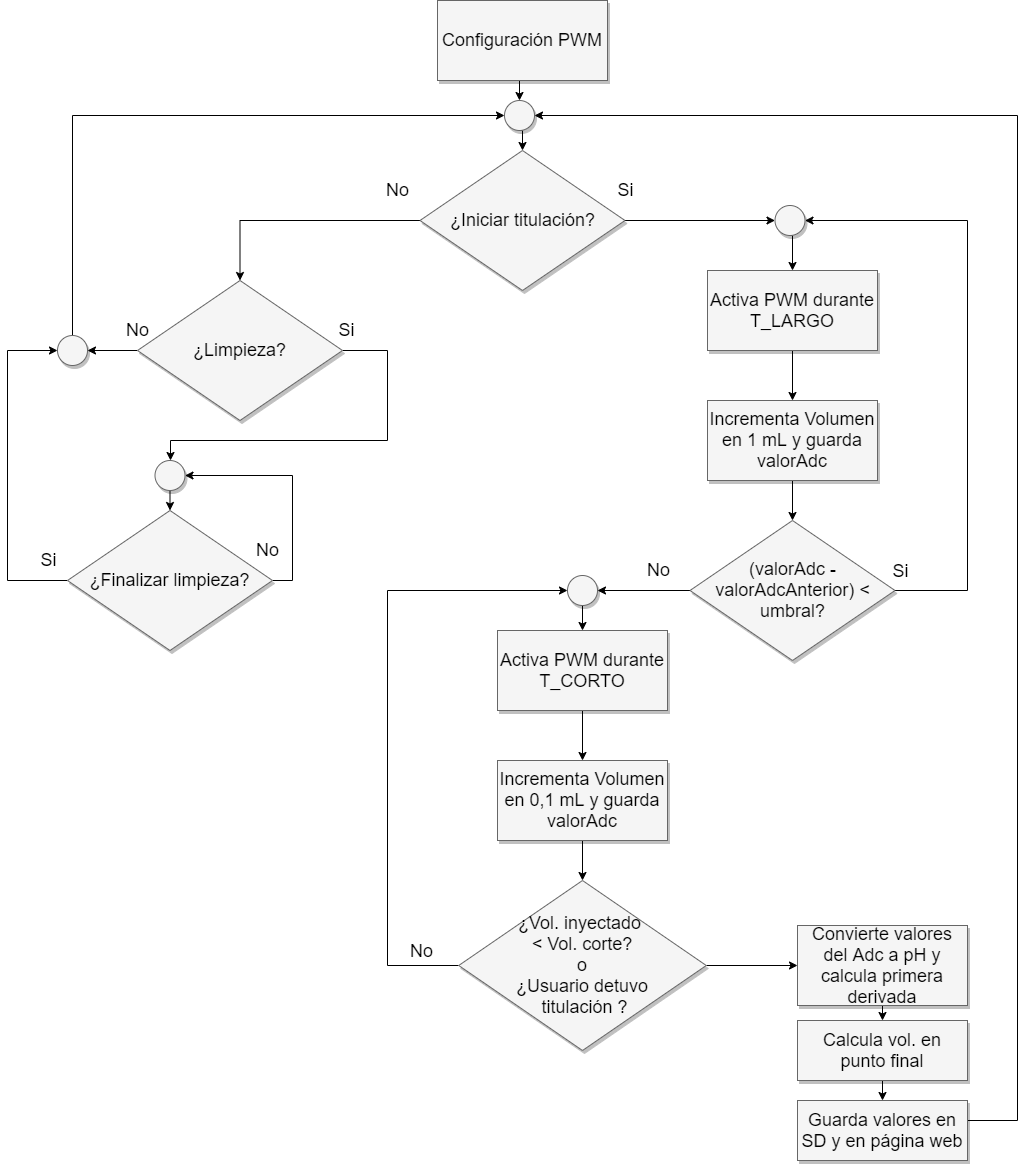
\includegraphics[width=1.0\textwidth]{./Figures/motorBomba.png}
	\caption{Diagrama de flujo de la tarea de control de la bomba.}
	\label{fig:flujoBomba}
\end{figure}

Ya definidas las configuraciones y los tiempos para cada cantidad del volumen, el proceso de titulación inicia con la activación del PWM que produce el giro de la bomba hasta alcanzar la cantidad de 1 mL de titulante inyectado. Llegado a este punto, se produce una espera de 5 segundos y luego se almacena el valor leído por la tarea del electrodo junto con la cantidad de volumen acumulado. El proceso se repite hasta que la diferencia entre las dos ultimas mediciones del electrodo supere un umbral, equivalente a aproximadamente 0,2 de pH. A partir de este momento, se modifica la cantidad de volumen inyectado a 0,1 mL pero el resto del procedimiento es el mismo. Una vez alcanzado el volumen de corte, o si el usuario presiona el boton de finalizar, la bomba se detiene y se llama a una función que calcula el valor de pH para cada valor almacenado en el arreglo de mediciones del electrodo. Luego, se calcula el valor de la primera derivada del pH respecto al volumen para cada uno de los valores del arreglo y se determina el volumen en el punto final en base al valor máximo de la primera derivada. Todos los valores son almacenados en la memoria micro SD y en la página web. Finalmente, el valor de volumen en el punto final es mostrado en la pantalla.


%----------------------------------------------------------------------------------------
\section{Interfaz de usuario}

La interfaz de usuario permite el acceso a todas las configuraciones y funciones que presenta el titulador. Está implementada a través de una pantalla táctil que permite navegar por un menú de diferentes pantallas, que fueron implementadas mediante la máquina de estados de la figura \ref{fig:MEFmenu}.

La máquina de estados se ejecuta en el ATMega328p y cada estado tiene una pantalla gráfica asociada con botones táctiles que permiten navegar entre las diferentes opciones. Por ejemplo, desde el menú inicial se puede acceder al menú de titulación a través del botón TITULAR.

\begin{figure}[htbp]
	\centering
	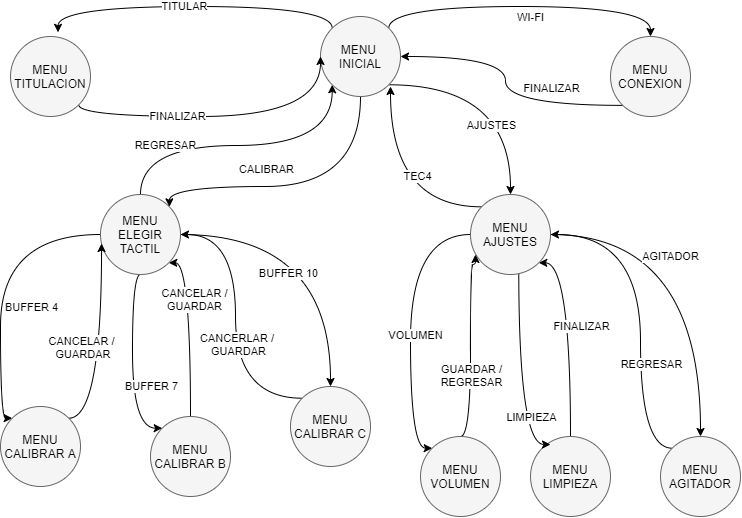
\includegraphics[width=1.0\textwidth]{./Figures/MEFmenu.png}
	\caption{Máquina de estados del menú de usuario.}
	\label{fig:MEFmenu}
\end{figure}

A continuación se listan las características de cada uno de los estados:

\begin{itemize}
\item Menú inicial: es el estado en el cual se ingresa cuando se inicia el programa. Desde aquí se puede acceder a la calibración, a la titulación, al menú de ajustes y al menú de conexión.
\item Menú elegir \textit{buffer}: se utiliza para elegir el \textit{buffer}  con el cual se desea calibrar. Para completar el proceso de calibración de manera correcta, se debe ingresar en cada uno de los tres \textit{buffers}. Al presionar REGRESAR se envía por UART que el proceso de calibración finalizó para que el ESP32 actualice la función correspondiente al cálculo del valor de pH.
\item Menú calibrar A: es el estado en el cual se calibra usando el \textit{buffer} de pH 4. En este estado el ATmega328p se comunica con el ESP32 para solicitarle el valor actual de pH. Este valor sirve como referencia para que el usuario presione GUARDAR una vez que la lectura sea estable. Al presionar GUARDAR, se envía la confirmación al ESP32 para que actualice el valor correspondiente al \textit{buffer} de pH 4, y se regresa al menú de elegir \textit{buffer}. En caso de presionar regresar, vuelve al menú pero sin enviar la confirmación al ESP32.
\item Menú calibrar B: es el estado en el cual se calibra usando el \textit{buffer} de pH 7, y sigue el mismo procedimiento que el menú calibrar A.
\item Menú calibrar C: es el estado en el cual se calibra usando el \textit{buffer} de pH 10, y sigue el mismo procedimiento que el menú calibrar A.
\item Menú titulación: es el estado en el cual se realiza el proceso de titulación, por ende, se envía un comando al ESP32 para que se ejecute la función de titulación dentro de la tarea de la bomba.
\item Menú ajustes: es el estado que permite acceder a varias configuraciones.
\item Menú volumen: es el estado que permite seleccionar el volumen de corte. Cuando se ingresa a este, se envía un comando al ESP32 para consultar el volumen de corte actual y mostrarlo en pantalla. Mediante un botón + y otro botón - se puede variar de a 1 mL este valor. Luego al presionar GUARDAR se envía el nuevo valor al ESP32, mientras que si se presionar REGRESAR vuelve al menú anterior sin hacer cambios.
\item Menú limpieza: es el estado que permite purgar o limpiar las mangueras de la bomba.  Aquí se envía un comando al ESP32 para que ejecute la función de limpieza dentro de la tarea de la bomba.
\item Menú agitador: es el estado que permite habilitar o deshabilitar el uso del agitador. Tiene los botones ON y OFF que envian al ESP32 el comando correspondiente para activar o desactivar el agitador respectivamente.
\item Menú conexión: es el estado que permitirá, en futuras versiones, acceder a configuraciones de la conexión Wi-Fi. Actualmente muestra la pantalla correspondiente pero no ejecuta ninguna acción.
\end{itemize}

Como se mencionó anteriormente, la máquina de estados funciona dentro del ATmega328p y en algunos estados se produce una comunicación mediante la UART con el ESP32 para el intercambio de la información necesaria. Esta comunicación se realiza utilizando comandos que representan determinadas acciones, algunos de los cuales van acompañados de algún valor o requieren determinada respuesta. A continuación, se describe cada uno de los comandos implementados:

\begin{itemize}
	\item Comando ''A'': El ATmega328p le indica al ESP32 que inicie el proceso de calibración.
	\item Comando ''B'': El ATmega328p le indica al ESP32 que finalice el proceso de calibración. El ESP32 calcula la pendiente y la ordenada al origen de la ecuación \ref{eq:conversionPh}.
	\item Comando ''C'': El ATmega328p le indica al ESP32 que convierta el valorAdc a pH y lo devuelva como respuesta.
	\item Comando ''D'': El ATmega328p le indica al ESP32 que el usuario guarde el valor actual de valorAdc como valor de calibración del \textit{buffer} de pH 4.
	\item Comando ''E'': El ATmega328p le indica al ESP32 que el usuario guarde el valor actual de valorAdc como valor de calibración del \textit{buffer} de pH 7.
	\item Comando ''F'': El ATmega328p le indica al ESP32 que el usuario guarde el valor actual de valorAdc como valor de calibración del \textit{buffer} de pH 10.
	\item Comando ''G'': El ATmega328p le indica al ESP32 que inicie el proceso de titulación.
	\item Comando ''I'': El ATmega328p le indica al ESP32 que finalice el proceso de titulación, porque el usuario lo seleccionó.  
	\item Comando ''J'': El ESP32 le indica al ATmega328p le indica al ESP32 el proceso de titulación finalizó, porque se alcanzó el volumen de corte.
	\item Comando ''K'': El ATmega328p le indica al ESP32 que inicie el proceso de limpieza.
	\item Comando ''L'': El ATmega328p le indica al ESP32 que finalice el proceso de limpieza.
	\item Comando ''M'': El ATmega328p le indica al ESP32 devuelva como respuesta el valor actual de volumen de corte.
	\item Comando ''N'': El ATmega328p le envía al ESP32 el valor de volumen de corte ingresado por el usuario.
	\item Comando ''P'': El ATmega328p le indica al ESP32 que habilite el agitador.
	\item Comando ''Q'': El ATmega328p le indica al ESP32 que deshabilite el agitador.
\end{itemize}



%----------------------------------------------------------------------------------------
\section{Almacenamiento de datos}

El almacenamiento de datos es una característica importante en este tipo de dispositivos ya que permite registrar los resultados de cada titulación para su posterior análisis en una computadora. Como método de almacenamiento se decidió utilizar una memoria del tipo micro SD, para sacar provecho del módulo que trae integrado la placa MCUFRIEND.

La API ESP-IDF incorpora funciones de alto nivel para la configuración, lectura y escritura de memorias SD a través del bus SPI. Para este trabajo se creó un módulo de \textit{firmware}, formado por un archivo denominado sd.c asociado al archivo sd.h, que ofrece funciones para inicializar la SD y escribir en ella.

La función inicializarSD se llama al inicio desde la función principal, previo a la creación de tareas, y hace la configuración inicial para habilitar el uso de la memoria micro SD. Dentro de ella, se hace el llamado a  la función spi\_bus\_initialize que inicia el bus SPI con las configuraciones de pines y velocidad, entre otras necesarias para la comunicación. Luego se realiza el llamado a esp\_vfs\_fat\_sdspi\_mount que especifica que sobre el bus SPI se monta una memoria del tipo SD que funciona con el sistema de archivos FAT.

La función para escribir en el archivo es accedida desde la tarea de la bomba para almacenar los datos correspondientes al volumen inyectado y pH y, además, el resultado del volumen en el punto final. El detalle de esta función se muestra en el pseudocódigo \ref{cod:escribeSD}. En la línea 1 se abre un archivo y en caso de que no se produzca un error, se procede a la escritura (línea 5) y finalmente se cierra el archivo (línea 6).

\begin{lstlisting}[label=cod:escribeSD,caption=Pseudocódigo de la función que escribe en la memoria SD.]
    FILE* f = fopen("TITULAR.txt", "a"); //Abre el archivo
    if (f == NULL) {
        return ERROR;
    }
    fprintf(f, "%s",dato);
    fclose(f);
    return OK;
\end{lstlisting}


%----------------------------------------------------------------------------------------
\section{Servidor web}

Para el desarrollo del prototipo se elaboró una página web que se almacena en la memoria flash del ESP32 y que se puede acceder a través de una conexión de área local gracias a la conexión Wi-Fi de la que dispone el módulo. En el código \ref{cod:servidorWeb} se muestra el pseudocódigo donde se encuentran las principales funciones que se utilizan para la conexión Wi-Fi y para la creación del servidor web.

\begin{lstlisting}[label=cod:servidorWeb,caption=Pseudocódigo del servidor web.]
main (){
	//...
	iniciarWiFi();
	iniciarServidorWeb();
	//...
}

//...

void iniciarWiFi()
{
	esp_wifi_init(); //Inicializa el stack de Wi-Fi con configuraciones por defecto
	esp_wifi_set_mode(ESTACION); //Configura el modo estacion
	esp_wifi_set_config(wifi_config); //Configura nombre de red del AP y contrasena
	esp_wifi_start(); //Realiza la conexion Wi-Fi
	registraHandlerDeEventos();
}

iniciarServidorWeb()
{
	if(httpd_start(configuraciones) = OK) //Crea un servidor HTTP
	{
		httpd_register_uri_handler(paginaHandler); //registra una pagina
	}
	
}

paginaHandler() //evento que se ejecuta cuando alguien accede a la pagina
{
	//Codigo HTML de la pagina que contiene el volumen en el punto final
	//y una tabla del volumen inyectado y pH
}

\end{lstlisting}

La función iniciarWiFi de la línea 10 se encarga de habilitar la conexión Wi-Fi en modo estación, con el nombre de la red y la contraseña del punto de acceso al cual se desea conectar. En la línea 16 registra eventos que se ejecutan cuando hay un cambio de ip o se produce un corte en la conexión, y tienen como objetivo restablecer la conexión.

La función iniciarServidorWeb de la línea 20 inicia un servidor HTTP con las configuraciones por defecto que ofrece la API y registra un evento asociado a la página web. Este evento se ejecuta cuando un cliente, conectado a la red local, intenta establecer la conexión mediante la ip asociada al ESP32. El controlador del evento ejecuta la función  de la línea 28 que actualiza la página web con los datos obtenidos en el último proceso de titulación.

%----------------------------------------------------------------------------------------
\section{Esquemáticos y PCB}

El diseño de los esquemáticos y del circuito impreso fueron realizados mediante la herramienta KiCad \citep{WEBSITE:9}. En la figura \ref{fig:esquematicoESP} se observan la fuente de alimentación y las conexiones asociadas al ESP32. La fuente de alimentación consta de un regulador de tensión de 5 V y su entrada proviene de una fuente externa de 12 V de corriente continua.

El ESP32 se conecta al módulo pH4502C mediante divisores resistivos para adaptar tensiones. Utiliza dos pines GPIO para la conexión al módulo DVR8825, un pin GPIO para la conexión al \textit{driver} del agitador, cuatro pines para la comunicación SPI con el módulo lector de tarjetas micro SD y dos pines para la comunicación UART con el ATmega328p. Además, los pines sin uso están conectados a tiras de pines para aplicaciones futuras.

\begin{figure}[htbp]
	\centering
	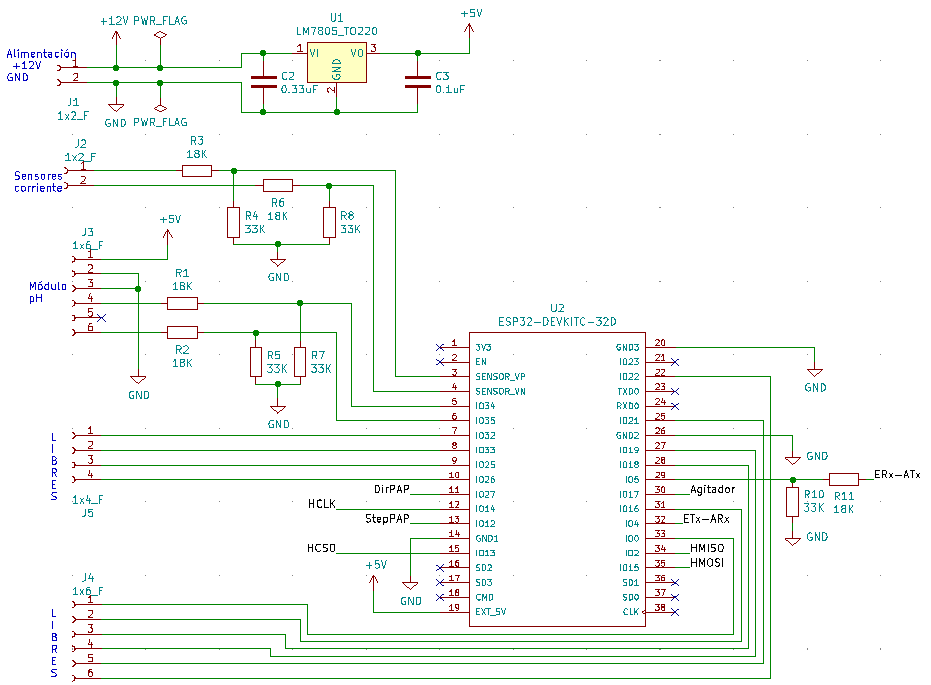
\includegraphics[width=1.0\textwidth]{./Figures/esquematicoESP.png}
	\caption{Diseño esquemático de las conexiones del ESP32.}
	\label{fig:esquematicoESP}
\end{figure}

La figura \ref{fig:esquematicoAtmega} muestra las conexiones del ATmega328p con los pines de control y datos de la pantalla táctil, asi como también los componentes mínimos necesarios para el funcionamiento del microcontrolador.

\begin{figure}[htbp]
	\centering
	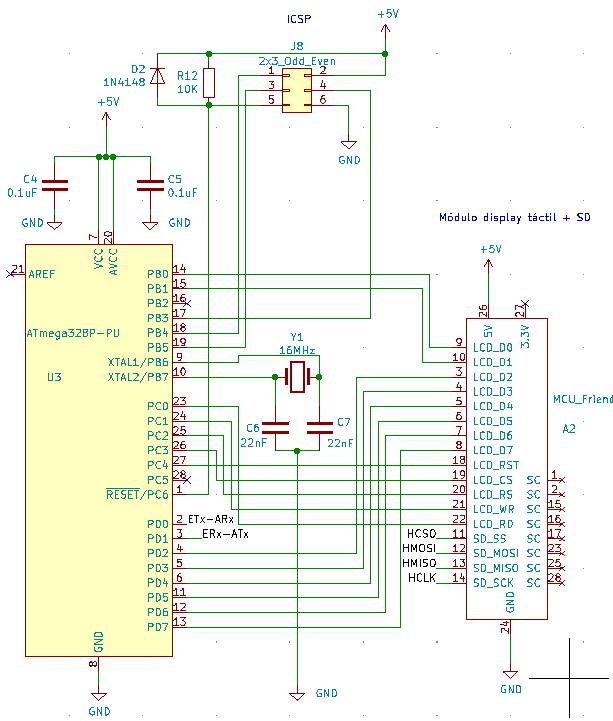
\includegraphics[width=0.6\textwidth]{./Figures/esquematicoAtmega.png}
	\caption{Diseño esquemático de las conexiones del ATmega328p.}
	\label{fig:esquematicoAtmega}
\end{figure}

El \textit{driver} DVR8825 tiene conectado un \textit{dip switch} que permite establecer por hardware el valor de configuración de \textit{microsteping}. Además, tiene el conector para los cables de las bobinas del motor. El \textit{driver} del agitador está formado por un transistor BJT en configuración común \cite{BOOK:3}. Estos circuitos están representados en la figura \ref{fig:esquematicoMotores}.

\begin{figure}[htbp]
	\centering
	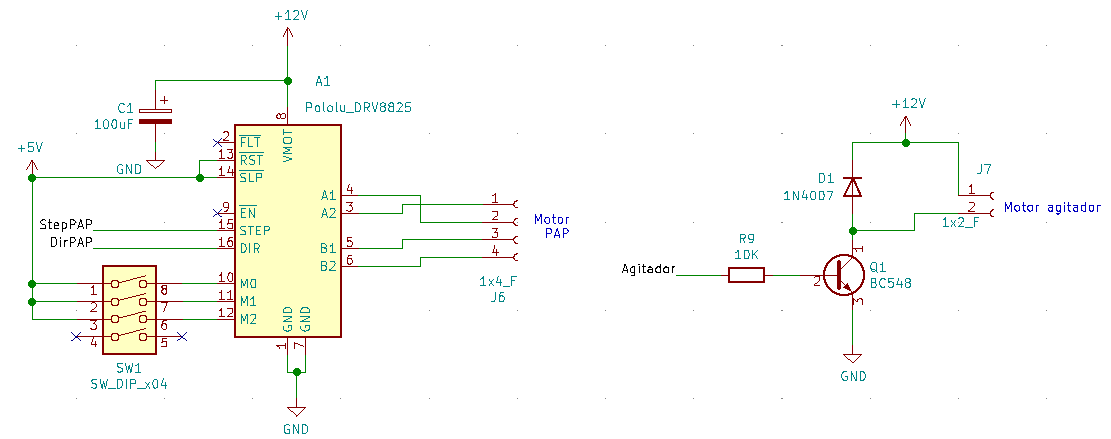
\includegraphics[width=1.0\textwidth]{./Figures/esquematicoMotores.png}
	\caption{Diseño esquemático de los drivers de la bomba y del agitador.}
	\label{fig:esquematicoMotores}
\end{figure}

El circuito impreso es una placa de 75 x 150 mm de dimensiones, diseñada en simple faz, y tiene como función la conexión de todos los módulos utilizados. En la figura \ref{fig:pcb3D} se observa el modelo 3D, mientras que en la figura \ref{fig:pcbPrototipo} se muestra una imagen del PCB construido de manera casera.


\begin{figure}[htbp]
	\centering
	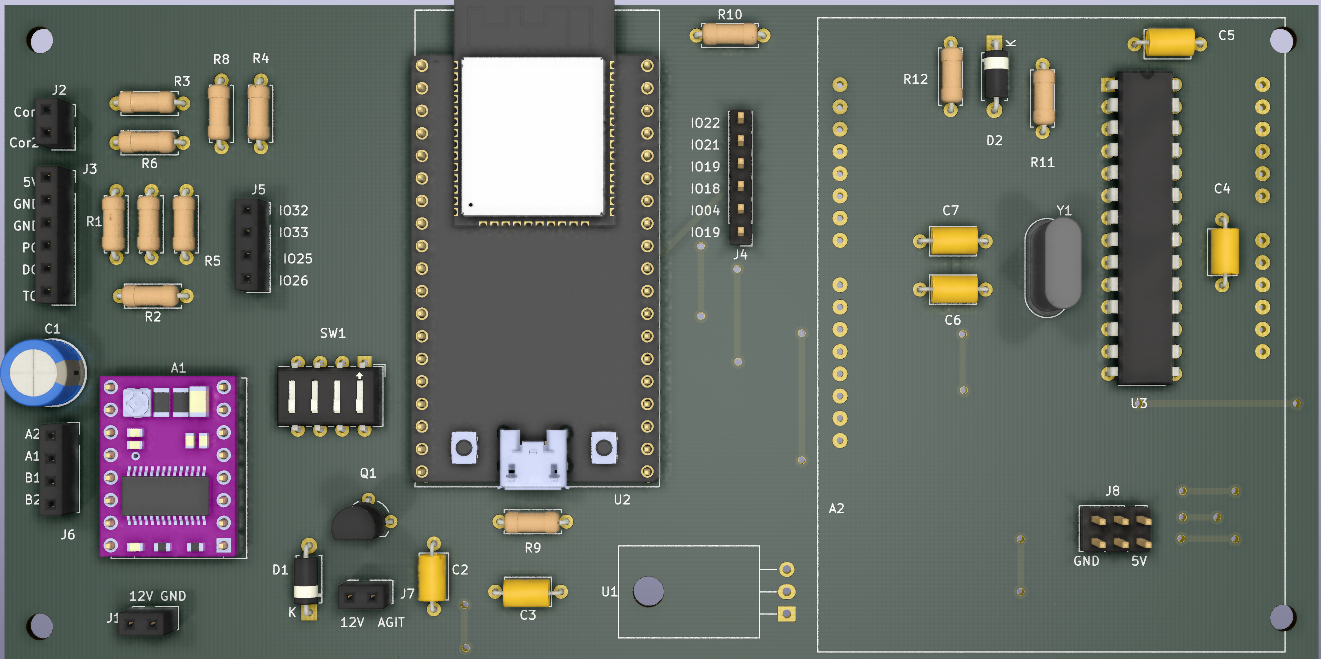
\includegraphics[width=0.9\textwidth]{./Figures/pcb3D.png}
	\caption{Modelo 3D del PCB.}
	\label{fig:pcb3D}
\end{figure}

\begin{figure}[htbp]
	\centering
	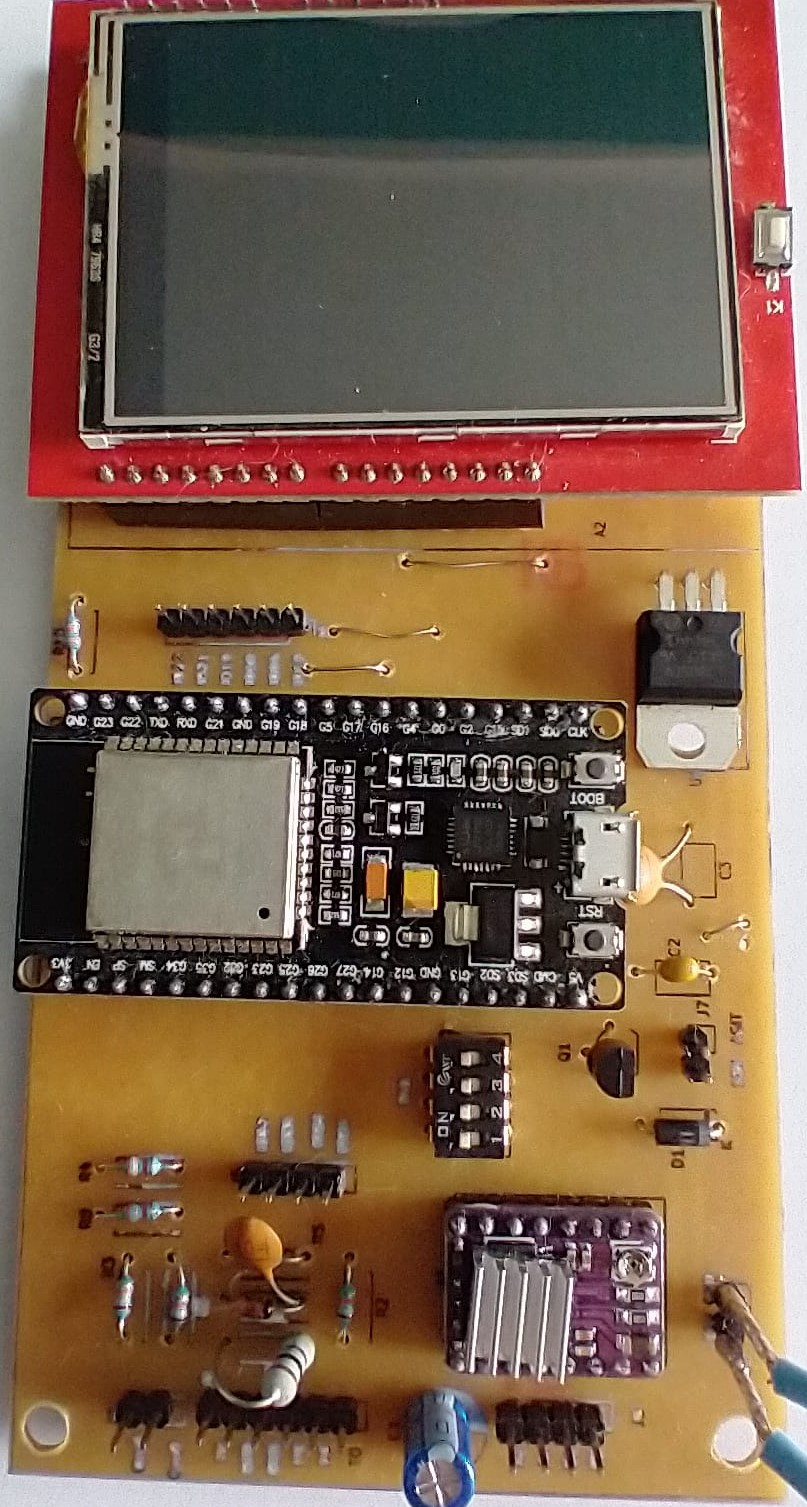
\includegraphics[width=0.5\textwidth]{./Figures/pcbPrototipo.jpeg}
	\caption{Prototipo final.}
	\label{fig:pcbPrototipo}
\end{figure}


% Chapter Template

\chapter{Ensayos y resultados} % Main chapter title

\label{Chapter4} % Change X to a consecutive number; for referencing this chapter elsewhere, use \ref{ChapterX}

%----------------------------------------------------------------------------------------
En este capítulo se muestran los principales ensayos realizados y sus resultados, para verificar el cumplimiento de los requisitos. Además, se incluye un caso de uso completo.

%----------------------------------------------------------------------------------------
%	SECTION 1
%----------------------------------------------------------------------------------------

\section{Pruebas unitarias}
\label{sec:pruebasUnitarias}

\subsection{Calibración del electrodo}

Para la validación del proceso de calibración del electrodo se utilizó el banco de pruebas que muestra la figura \ref{fig:bancoPruebasCalibracion}, y se procedió a realizar el proceso de calibración.

\begin{figure}[htbp]
	\centering
	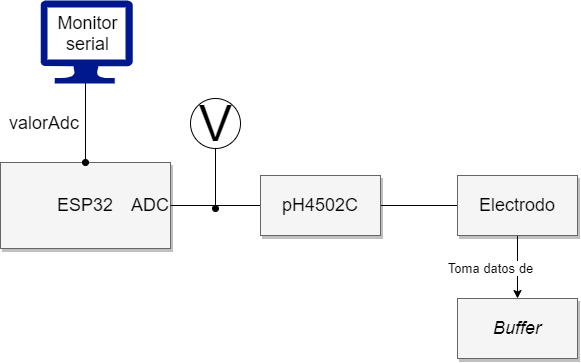
\includegraphics[width=0.7\textwidth]{./Figures/bancoPruebasCalibracion.png}
	\caption{Banco de pruebas para la calibración del electrodo.}
	\label{fig:bancoPruebasCalibracion}
\end{figure}

La tabla \ref{tab:ensayoCalibracion} muestra las mediciones correspondientes a la diferencia de potencial entregada por módulo pH4502C y al valor leído por el ADC para cada unos de los valores de los \textit{buffers}, en un ambiente con temperatura de 25 °C.

\begin{table}[h]
	\centering
	\caption[Resultados calibración]{Resultados obtenidos durante el proceso de calibración}
	\begin{tabular}{l c c }    
		\toprule
		\textbf{\textit{Buffer} [pH]} & \textbf{Salida pH4602C [V] }	&    \textbf{Lectura ADC}  \\
		\midrule
		4 	& 2,635 & 3050 \\		
		7	& 2,172 & 2455 \\
		10	& 1,877 & 2120 \\
		\bottomrule
		\hline
	\end{tabular}
	\label{tab:ensayoCalibracion}
\end{table}

A partir de los datos obtenidos, se puede graficar la recta de ajuste que relaciona el valor de pH con el valor de medido por el ADC, como se muestra en la figura \ref{fig:rectaADC}. Los valores de pendiente y ordenada al origen calculados en el ESP32 fueron visualizados por el monitor serial, y se obtuvo -0,0063 para el valor de la pendiente m, y 22,98 para el valor de la ordenada al origen b. 

\begin{figure}[htbp]
	\centering
	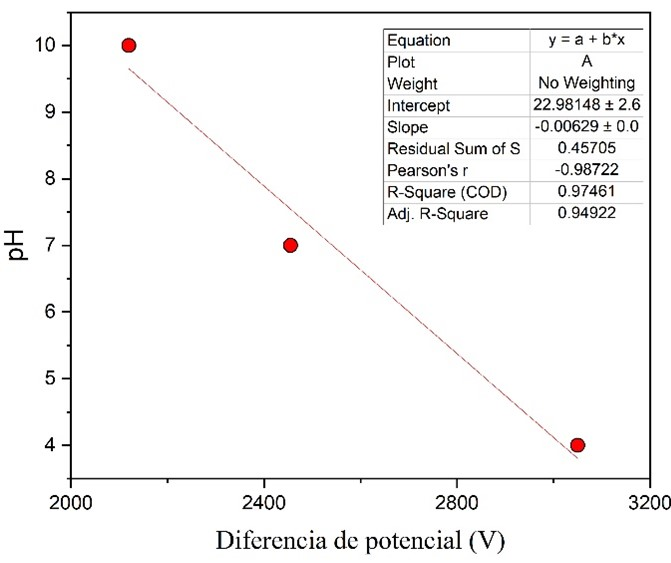
\includegraphics[width=0.7\textwidth]{./Figures/rectaADC.jpg}
	\caption{Relación entre el pH y el valor convertido por el ADC.}
	\label{fig:rectaADC}
\end{figure}

Luego de repetir el ensayo, se obtuvo que el error en la medición del potencial de salida del módulo pH4502C es de +/- 1 mV y luego de la conversión a pH el error es de +/- 0,1 pH a temperatura ambiente. 

\subsection{Calibración del volumen inyectado por la bomba}

En el diseño del prototipo, el control de bomba se realiza utilizando un esquema de lazo abierto, es decir que, cuando se inyecta líquido, el microcontrolador  no realiza una medición del caudal o del volumen que fue desplazado. A raíz de esto, surge la necesidad de establecer una relación entre la cantidad de pasos que realiza el motor y la cantidad de volumen que inyecta la bomba, para así poder tener una unidad de medida y verificar si cumple con los requerimientos establecidos. Esta relación es difícil de obtener de manera teórica mediante el uso de modelos, por lo que se decidió realizar una serie de dosificaciones de un líquido de densidad conocida, y pesar la cantidad dosificada para determinar el volumen. En banco de pruebas utilizado para realizar este ensayo se muestra en la figura \ref{fig:bancoPruebasBomba}. En este proceso el fluido a dosificar fue agua de red domiciliaria, con una densidad estimada de 1 g/mL y se utilizó una balanza de dos decimales con un error de ±0,01 g, recogiendo el fluido en un vaso de precipitado previamente tarado.

\begin{figure}[htbp]
	\centering
	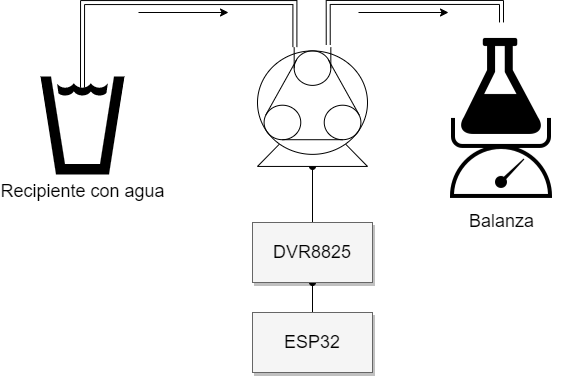
\includegraphics[width=0.7\textwidth]{./Figures/bancoPruebasBomba.png}
	\caption{Banco de pruebas para la calibración de la bomba.}
	\label{fig:bancoPruebasBomba}
\end{figure}

Se realizaron 10 dosificaciones, cada una de las cuales implicó una cantidad de 2500 pasos para el motor, a una velocidad constante de 93,75 rpm. Se registró el peso y se taró nuevamente la balanza para todas las dosificaciones. Esta relación entre el número de pasos y las mediciones de masa se muestra en la tabla \ref{tab:ensayoBomba}, y la serie de mediciones arroja un peso medio de 0,70 g con un desvío de ± 0,01 g.

\begin{table}[h]
	\centering
	\caption[Dosificaciones]{Dosificaciones para el cálculo de volumen por paso.}
	\begin{tabular}{l c }    
		\toprule
		\textbf{Número de dosificación} & \textbf{Peso [g] } \\
		\midrule
		1 	& 0,69 \\	
		2	& 0,70 \\
		3	& 0,69 \\
		4	& 0,69 \\
		5	& 0,71 \\
		6	& 0,70 \\
		7	& 0,69 \\
		8	& 0,69 \\
		9	& 0,70 \\
		10	& 0,69 \\
		\bottomrule
		\hline
	\end{tabular}
	\label{tab:ensayoBomba}
\end{table}

\section{Validación y verificación}
\label{sec:validacionVerificacion}

Para la validación del prototipo se desarrolló un caso de uso que incluyó los siguientes pasos:
\begin{itemize}
	\item Calibración del electrodo con los 3 \textit{buffers}.
	\item Configuración del volumen de corte.
	\item Proceso de limpieza.
	\item Titulación de 50 mL de HCI 0,0500 M con NaOH 0,100 M.
	\item Visualización de resultados en memoria micro SD y página web.
\end{itemize}




 
% Chapter Template

\chapter{Conclusiones} % Main chapter title

\label{Chapter5} % Change X to a consecutive number; for referencing this chapter elsewhere, use \ref{ChapterX}


%----------------------------------------------------------------------------------------

En este capítulo se destacan los objetivos cumplidos con el trabajo realizado y se plantean los pasos a seguir para realizar mejoras futuras.

%----------------------------------------------------------------------------------------
%	SECTION 1
%----------------------------------------------------------------------------------------

\section{Resultados obtenidos }

Los objetivos y requerimientos planteados al inicio del proyecto fueron cumplidos en su totalidad. El tiempo de ejecución de las tareas fue similar al estimado, pero no pudo respetarse el cronograma debido a las restricciones por el COVID-19. Pese a estas demoras, luego de ajustados los plazos de entrega, las tareas fueron ejecutadas con normalidad en el tiempo estimado.

Además, es importante destacar el uso de los conocimientos y técnicas utilizadas en el desarrollo que fueron adquiridos en las asignaturas de la especialización:
\begin{itemize}
 \item Programación de microcontroladores: uso de máquinas de estados finitos en la interfaz de usuario.
 \item Sistemas operativos de tiempo real: uso de FreeRTOS para la ejecución de tareas con restricciones de tiempo en su ejecución.
 \item Protocolos de comunicación en sistemas embebidos: uso de protocolos y comunicaciones, como ser UART, SPI y Wi-Fi.
 \item Diseño de circuitos impresos: uso de técnicas de diseño de esquemáticos y circuitos impresos.
\end{itemize}

Por último, es importante destacar que se obtuvo un prototipo funcional que cumple con las funciones básicas de los tituladores comerciales y es accesible económicamente para universidades y laboratorios pequeños.

%----------------------------------------------------------------------------------------
%	SECTION 2
%----------------------------------------------------------------------------------------
\section{Trabajo futuro}

El siguiente paso a seguir es realizar mejoras funcionales respecto al \textit{firmware}. Por ejemplo la gráfica de pH respecto al tiempo debería ser de pH respecto al volumen. Además, se piensa agregar una opción para que el usuario pueda configurar la red Wi-Fi. Las principales mejoras respecto al hardware dependen de la inclusión de nuevos componentes. La utilización de un sensor de temperatura permitiría ajustar el valor de pH para muestras que no están a temperatura ambiente. Además, el uso de un sensor de flujo permitiría tener una medida del volumen inyectado y crear un sistema de control de lazo cerrado. 

%----------------------------------------------------------------------------------------
%	CONTENIDO DE LA MEMORIA  - APÉNDICES
%----------------------------------------------------------------------------------------

\appendix % indicativo para indicarle a LaTeX los siguientes "capítulos" son apéndices

% Incluir los apéndices de la memoria como archivos separadas desde la carpeta Appendices
% Descomentar las líneas a medida que se escriben los apéndices

%\include{Appendices/AppendixA}
%\include{Appendices/AppendixB}
%\include{Appendices/AppendixC}

%----------------------------------------------------------------------------------------
%	BIBLIOGRAPHY
%----------------------------------------------------------------------------------------

\Urlmuskip=0mu plus 1mu\relax
\raggedright
\printbibliography[heading=bibintoc]

%----------------------------------------------------------------------------------------

\end{document}  
